%########################### Preferences #################################
\usepackage{amsmath, amsfonts, amssymb}
%\usepackage[margin=1.2in,headsep=.5in]{geometry}
%\setpapersize{letterpaper}
\usepackage[margin=1in]{geometry}
\usepackage{vmargin} %reduce to amount of white space on the page
\usepackage{longtable}
\usepackage{morefloats}
\usepackage{enumitem}
\usepackage{xcolor}
%\usepackage{tcolorbox}
\usepackage{totpages}
\usepackage{pdflscape}
\usepackage{minted}
\usepackage{listings}
% Code listing settings
\lstset{
    language=Python,
    basicstyle=\ttfamily\small,
    keywordstyle=\color{blue},
    commentstyle=\color{green},
    stringstyle=\color{red},
    showstringspaces=false,
    breaklines=true,
    frame=single,
    numbers=left,
    numberstyle=\tiny\color{gray}
}
\usepackage{listingsutf8}

% ********* Font definiton ************
\usepackage[T1]{fontenc}
\usepackage[utf8]{inputenc}
\usepackage{pmboxdraw}  % For box drawing characters
%\usepackage{fontspec}
%\setmainfont{Latin Modern Roman} % Or any other font with good Unicode support
\usepackage{fontawesome5}
\usepackage{pifont} 

% ********* Macro for Models ************
% ============================================
% model_template_setup.tex
% ============================================
% Defines \SetupModelTemplate{ModelWord} macro
% Maps generic template commands (\M...) to model-specific commands (\ModelX...)
%
% Usage in model chapters:
%   \SetupModelTemplate{One}   % For Model 1
%   \SetupModelTemplate{Two}   % For Model 2
%   \SetupModelTemplate{Five}  % For Model 5
%   etc.
%
% After calling this macro, the template can use generic commands like:
%   \MRSquaredTest   → maps to \ModelOneRSquaredTest (for Model 1)
%   \MRMSETest       → maps to \ModelOneRMSETest (for Model 1)
%   etc.
% ============================================
% Usage Example:
% ============================================
% In 3Alternative-1-CurrentUpdated.tex (Model 1):
%
% \chapter{Model 1: Re-evaluation of Model 5b}
% % Model 1 Calibrated Values
% Generated: 2025-10-02 01:58:23.185499
% Model: Linear with Outlier Removal

% Core Metrics
\renewcommand{\ModelOneRSquaredTrain}{0.2383}
\renewcommand{\ModelOneRSquaredTest}{0.2178}
\renewcommand{\ModelOneRMSETrain}{39,238}
\renewcommand{\ModelOneRMSETest}{39,500}
\renewcommand{\ModelOneMAETrain}{27,831}
\renewcommand{\ModelOneMAETest}{27,912}
\renewcommand{\ModelOneMAPETrain}{85.2}
\renewcommand{\ModelOneMAPETest}{84.8}
\renewcommand{\ModelOneCVMean}{0.2372}
\renewcommand{\ModelOneCVStd}{0.0196}
\renewcommand{\ModelOneWithinOneK}{2.4}
\renewcommand{\ModelOneWithinTwoK}{4.9}
\renewcommand{\ModelOneWithinFiveK}{15.8}
\renewcommand{\ModelOneWithinTenK}{28.5}
\renewcommand{\ModelOneWithinTwentyK}{49.5}
\renewcommand{\ModelOneTrainingSamples}{27,339}
\renewcommand{\ModelOneTestSamples}{6,834}

% Subgroup Metrics
\renewcommand{\ModelOneSubgrouplivingFHN}{5,941}
\renewcommand{\ModelOneSubgrouplivingFHRSquared}{0.222}
\renewcommand{\ModelOneSubgrouplivingFHRMSE}{39,928}
\renewcommand{\ModelOneSubgrouplivingFHBias}{-7,487}
\renewcommand{\ModelOneSubgrouplivingILSLN}{893}
\renewcommand{\ModelOneSubgrouplivingILSLRSquared}{0.179}
\renewcommand{\ModelOneSubgrouplivingILSLRMSE}{36,524}
\renewcommand{\ModelOneSubgrouplivingILSLBias}{-3,272}
\renewcommand{\ModelOneSubgroupageAgeUnderTwentyOneN}{694}
\renewcommand{\ModelOneSubgroupageAgeUnderTwentyOneRSquared}{0.138}
\renewcommand{\ModelOneSubgroupageAgeUnderTwentyOneRMSE}{34,649}
\renewcommand{\ModelOneSubgroupageAgeUnderTwentyOneBias}{-8,152}
\renewcommand{\ModelOneSubgroupageAgeTwentyOneToThirtyN}{1,797}
\renewcommand{\ModelOneSubgroupageAgeTwentyOneToThirtyRSquared}{0.161}
\renewcommand{\ModelOneSubgroupageAgeTwentyOneToThirtyRMSE}{44,751}
\renewcommand{\ModelOneSubgroupageAgeTwentyOneToThirtyBias}{-7,785}
\renewcommand{\ModelOneSubgroupageAgeThirtyOnePlusN}{4,343}
\renewcommand{\ModelOneSubgroupageAgeThirtyOnePlusRSquared}{0.218}
\renewcommand{\ModelOneSubgroupageAgeThirtyOnePlusRMSE}{37,876}
\renewcommand{\ModelOneSubgroupageAgeThirtyOnePlusBias}{-6,391}
\renewcommand{\ModelOneSubgroupcostQOneLowN}{1,709}
\renewcommand{\ModelOneSubgroupcostQOneLowRSquared}{-10.000}
\renewcommand{\ModelOneSubgroupcostQOneLowRMSE}{31,272}
\renewcommand{\ModelOneSubgroupcostQOneLowBias}{+24,162}
\renewcommand{\ModelOneSubgroupcostQTwoN}{1,708}
\renewcommand{\ModelOneSubgroupcostQTwoRSquared}{-6.029}
\renewcommand{\ModelOneSubgroupcostQTwoRMSE}{20,461}
\renewcommand{\ModelOneSubgroupcostQTwoBias}{+9,755}
\renewcommand{\ModelOneSubgroupcostQThreeN}{1,708}
\renewcommand{\ModelOneSubgroupcostQThreeRSquared}{-4.117}
\renewcommand{\ModelOneSubgroupcostQThreeRMSE}{26,401}
\renewcommand{\ModelOneSubgroupcostQThreeBias}{-13,739}
\renewcommand{\ModelOneSubgroupcostQFourHighN}{1,709}
\renewcommand{\ModelOneSubgroupcostQFourHighRSquared}{-2.230}
\renewcommand{\ModelOneSubgroupcostQFourHighRMSE}{64,390}
\renewcommand{\ModelOneSubgroupcostQFourHighBias}{-47,917}

% Variance Metrics
\renewcommand{\ModelOneCVActual}{1.010}
\renewcommand{\ModelOneCVPredicted}{0.692}
\renewcommand{\ModelOnePredictionInterval}{152,432}
\renewcommand{\ModelOneBudgetActualCorr}{0.498}
\renewcommand{\ModelOneQuarterlyVariance}{87.9}
\renewcommand{\ModelOneAnnualAdjustmentRate}{92.4}

% Population Scenarios
\renewcommand{\ModelOnePopcurrentbaselineClients}{32,188}
\renewcommand{\ModelOnePopcurrentbaselineAvgAlloc}{37,280}
\renewcommand{\ModelOnePopcurrentbaselineWaitlistChange}{+0}
\renewcommand{\ModelOnePopcurrentbaselineWaitlistPct}{+0.0}
\renewcommand{\ModelOnePopmodelbalancedClients}{32,831}
\renewcommand{\ModelOnePopmodelbalancedAvgAlloc}{36,534}
\renewcommand{\ModelOnePopmodelbalancedWaitlistChange}{+643}
\renewcommand{\ModelOnePopmodelbalancedWaitlistPct}{+2.0}
\renewcommand{\ModelOnePopmodelefficiencyClients}{33,797}
\renewcommand{\ModelOnePopmodelefficiencyAvgAlloc}{35,416}
\renewcommand{\ModelOnePopmodelefficiencyWaitlistChange}{+1,609}
\renewcommand{\ModelOnePopmodelefficiencyWaitlistPct}{+5.0}
\renewcommand{\ModelOnePopcategoryfocusedClients}{27,359}
\renewcommand{\ModelOnePopcategoryfocusedAvgAlloc}{43,990}
\renewcommand{\ModelOnePopcategoryfocusedWaitlistChange}{-4,828}
\renewcommand{\ModelOnePopcategoryfocusedWaitlistPct}{-15.0}
\renewcommand{\ModelOnePoppopulationmaximizedClients}{37,016}
\renewcommand{\ModelOnePoppopulationmaximizedAvgAlloc}{32,434}
\renewcommand{\ModelOnePoppopulationmaximizedWaitlistChange}{+4,828}
\renewcommand{\ModelOnePoppopulationmaximizedWaitlistPct}{+15.0}

% Model 1 Specific Metrics
\renewcommand{\ModelOneOutliersRemoved}{2570}
\renewcommand{\ModelOneOutlierPercentage}{9.4}
\renewcommand{\ModelOneTransformation}{Square Root}
\renewcommand{\ModelOneNumFeatures}{26}
\renewcommand{\ModelOnePredictionFloor}{5,000}

% Feature Selection Specific Values
\renewcommand{\ModelOneFeatureSelection}{True}
\renewcommand{\ModelOneFiscalYears}{2024}
\renewcommand{\ModelOneMIScoreTop}{0.272}
\renewcommand{\ModelOneVarianceExplained}{89.0}

% \SetupModelTemplate{One}
% % ============================================
% model_template.tex
% ============================================
% Universal template for all models
% Uses generic \M... commands that get mapped to model-specific commands
% 
% IMPORTANT: Call \SetupModelTemplate{ModelWord} BEFORE inputting this file
% ============================================

\section{Performance Metrics}

\subsection{Overall Performance}

\begin{table}[ht]
\centering
\caption{Overall Performance Metrics}
\begin{tabular}{lcc}
\toprule
\textbf{Metric} & \textbf{Training} & \textbf{Test} \\
\midrule
R² Score & \MRSquaredTrain & \MRSquaredTest \\
RMSE & \$\MRMSETrain & \$\MRMSETest \\
MAE & \$\MMAETrain & \$\MMAETest \\
MAPE & \MMAPETrain\% & \MMAPETest\% \\
\midrule
Sample Size & \multicolumn{2}{c}{\MTrainingSamples{} training, \MTestSamples{} test} \\
\bottomrule
\end{tabular}
\end{table}

\subsection{Accuracy Bands}

\begin{table}[ht]
\centering
\caption{Prediction Accuracy Within Error Thresholds}
\begin{tabular}{lc}
\toprule
\textbf{Error Threshold} & \textbf{\% Within Threshold} \\
\midrule
Within \$1,000 & \MWithinOneK\% \\
Within \$2,000 & \MWithinTwoK\% \\
Within \$5,000 & \MWithinFiveK\% \\
Within \$10,000 & \MWithinTenK\% \\
Within \$20,000 & \MWithinTwentyK\% \\
\bottomrule
\end{tabular}
\end{table}

\subsection{Cross-Validation Results}

\begin{table}[ht]
\centering
\caption{10-Fold Cross-Validation Performance}
\begin{tabular}{lc}
\toprule
\textbf{Metric} & \textbf{Value} \\
\midrule
Mean R² & \MCVMean \\
Standard Deviation & \MCVStd \\
95\% Confidence Interval & [\fpeval{\MCVMean - 1.96*\MCVStd}, \fpeval{\MCVMean + 1.96*\MCVStd}] \\
\bottomrule
\end{tabular}
\end{table}

\newpage
\section{Subgroup Analysis}

\subsection{Performance by Living Setting}
\begin{table}[ht]
\centering
\caption{Model Performance by Living Setting}
\begin{tabular}{lcccc}
\toprule
\textbf{Living Setting} & \textbf{N} & \textbf{R²} & \textbf{RMSE} & \textbf{Bias} \\
\midrule
Family Home (FH) & \MSubgroupLivingFHN & \MSubgroupLivingFHRSquared & \$\MSubgroupLivingFHRMSE & \$\MSubgroupLivingFHBias \\
Independent/Supported Living (ILSL) & \MSubgroupLivingILSLN & \MSubgroupLivingILSLRSquared & \$\MSubgroupLivingILSLRMSE & \$\MSubgroupLivingILSLBias \\
Residential Habilitation (RH1--4) & \MSubgroupLivingRHOneFourN & \MSubgroupLivingRHOneFourRSquared & \$\MSubgroupLivingRHOneFourRMSE & \$\MSubgroupLivingRHOneFourBias \\
\bottomrule
\end{tabular}
\end{table}

\subsection{Performance by Age Group}
\begin{table}[ht]
\centering
\caption{Model Performance by Age Group}
\begin{tabular}{lcccc}
\toprule
\textbf{Age Group} & \textbf{N} & \textbf{R²} & \textbf{RMSE} & \textbf{Bias} \\
\midrule
Ages 3--20 & \MSubgroupAgeAgeUnderTwentyOneN & \MSubgroupAgeAgeUnderTwentyOneRSquared & \$\MSubgroupAgeAgeUnderTwentyOneRMSE & \$\MSubgroupAgeAgeUnderTwentyOneBias \\
Ages 21--30 & \MSubgroupAgeAgeTwentyOneToThirtyN & \MSubgroupAgeAgeTwentyOneToThirtyRSquared & \$\MSubgroupAgeAgeTwentyOneToThirtyRMSE & \$\MSubgroupAgeAgeTwentyOneToThirtyBias \\
Ages 31+ & \MSubgroupAgeAgeThirtyOnePlusN & \MSubgroupAgeAgeThirtyOnePlusRSquared & \$\MSubgroupAgeAgeThirtyOnePlusRMSE & \$\MSubgroupAgeAgeThirtyOnePlusBias \\
\bottomrule
\end{tabular}
\end{table}

\subsection{Performance by Cost Quartile}

\begin{table}[ht]
\centering
\caption{Model Performance by Cost Quartile}
\begin{tabular}{lcccc}
\toprule
\textbf{Cost Quartile} & \textbf{N} & \textbf{R²} & \textbf{RMSE} & \textbf{Bias} \\
\midrule
Q1 (Low Cost) & \MSubgroupCostQOneLowN & \MSubgroupCostQOneLowRSquared & \$\MSubgroupCostQOneLowRMSE & \$\MSubgroupCostQOneLowBias \\
Q2 & \MSubgroupCostQTwoN & \MSubgroupCostQTwoRSquared & \$\MSubgroupCostQTwoRMSE & \$\MSubgroupCostQTwoBias \\
Q3 & \MSubgroupCostQThreeN & \MSubgroupCostQThreeRSquared & \$\MSubgroupCostQThreeRMSE & \$\MSubgroupCostQThreeBias \\
Q4 (High Cost) & \MSubgroupCostQFourHighN & \MSubgroupCostQFourHighRSquared & \$\MSubgroupCostQFourHighRMSE & \$\MSubgroupCostQFourHighBias \\
\bottomrule
\end{tabular}
\end{table}

\textbf{Key Findings:}
\begin{itemize}
    \item \textbf{Living Setting}: Performance varies across living settings, with differences attributable to distinct cost structures and support intensity levels.
    \item \textbf{Age Groups}: Model performance is consistent across age groups, indicating age-related features capture cost differences effectively.
    \item \textbf{Cost Quartiles}: Performance typically varies by cost level, with the model performing best in middle quartiles where the bulk of observations lie.
\end{itemize}

\section{Variance and Stability Metrics}

\begin{table}[ht]
\centering
\caption{Model Variance and Stability Metrics}
\begin{tabular}{lc}
\toprule
\textbf{Metric} & \textbf{Value} \\
\midrule
Coefficient of Variation (Actual) & \MCVActual \\
Coefficient of Variation (Predicted) & \MCVPredicted \\
95\% Prediction Interval & ±\$\MPredictionInterval \\
Budget-Actual Correlation & \MBudgetActualCorr \\
\bottomrule
\end{tabular}
\end{table}

\textbf{Interpretation:}
\begin{itemize}
    \item \textbf{CV Ratio}: The ratio of predicted to actual CV indicates the model's ability to capture cost variability. Values close to 1.0 suggest the model accurately reflects population heterogeneity.
    \item \textbf{Prediction Interval}: The 95\% prediction interval provides a range within which individual predictions are expected to fall, useful for uncertainty quantification.
    \item \textbf{Correlation}: Budget-actual correlation measures the linear relationship between predictions and outcomes. High values ($>$ 0.80) indicate strong predictive validity.
\end{itemize}

\section{Population Impact Scenarios}

\begin{table}[ht]
\centering
\caption{Population Served Analysis --- \$1.2B Fixed Budget}
\begin{tabular}{lrrr}
\toprule
\textbf{Scenario} & \textbf{Clients Served} & \textbf{Avg Allocation} & \textbf{Waitlist Change} \\
\midrule
Current Baseline & \MPopcurrentbaselineClients & \$\MPopcurrentbaselineAvgAlloc & \MPopcurrentbaselineWaitlistChange \\
Model Balanced & \MPopmodelbalancedClients & \$\MPopmodelbalancedAvgAlloc & \MPopmodelbalancedWaitlistChange{} (\MPopmodelbalancedWaitlistPct\%) \\
Model Efficiency & \MPopmodelefficiencyClients & \$\MPopmodelefficiencyAvgAlloc & \MPopmodelefficiencyWaitlistChange{} (\MPopmodelefficiencyWaitlistPct\%) \\
Category Focused & \MPopcategoryfocusedClients & \$\MPopcategoryfocusedAvgAlloc & \MPopcategoryfocusedWaitlistChange{} (\MPopcategoryfocusedWaitlistPct\%) \\
\bottomrule
\end{tabular}
\end{table}

\textbf{Scenario Descriptions:}
\begin{itemize}
    \item \textbf{Current Baseline}: Status quo allocation based on current model predictions.
    \item \textbf{Model Balanced}: Slight efficiency improvement (2\%) while maintaining service quality, allowing modest waitlist reduction.
    \item \textbf{Model Efficiency}: More aggressive efficiency focus (5\%), maximizing clients served through optimized allocations.
    \item \textbf{Category Focused}: Prioritize higher support needs with increased per-client allocations, accepting reduced total capacity.
\end{itemize}

\section{Model Diagnostics}

\begin{figure}[ht]
    \centering
    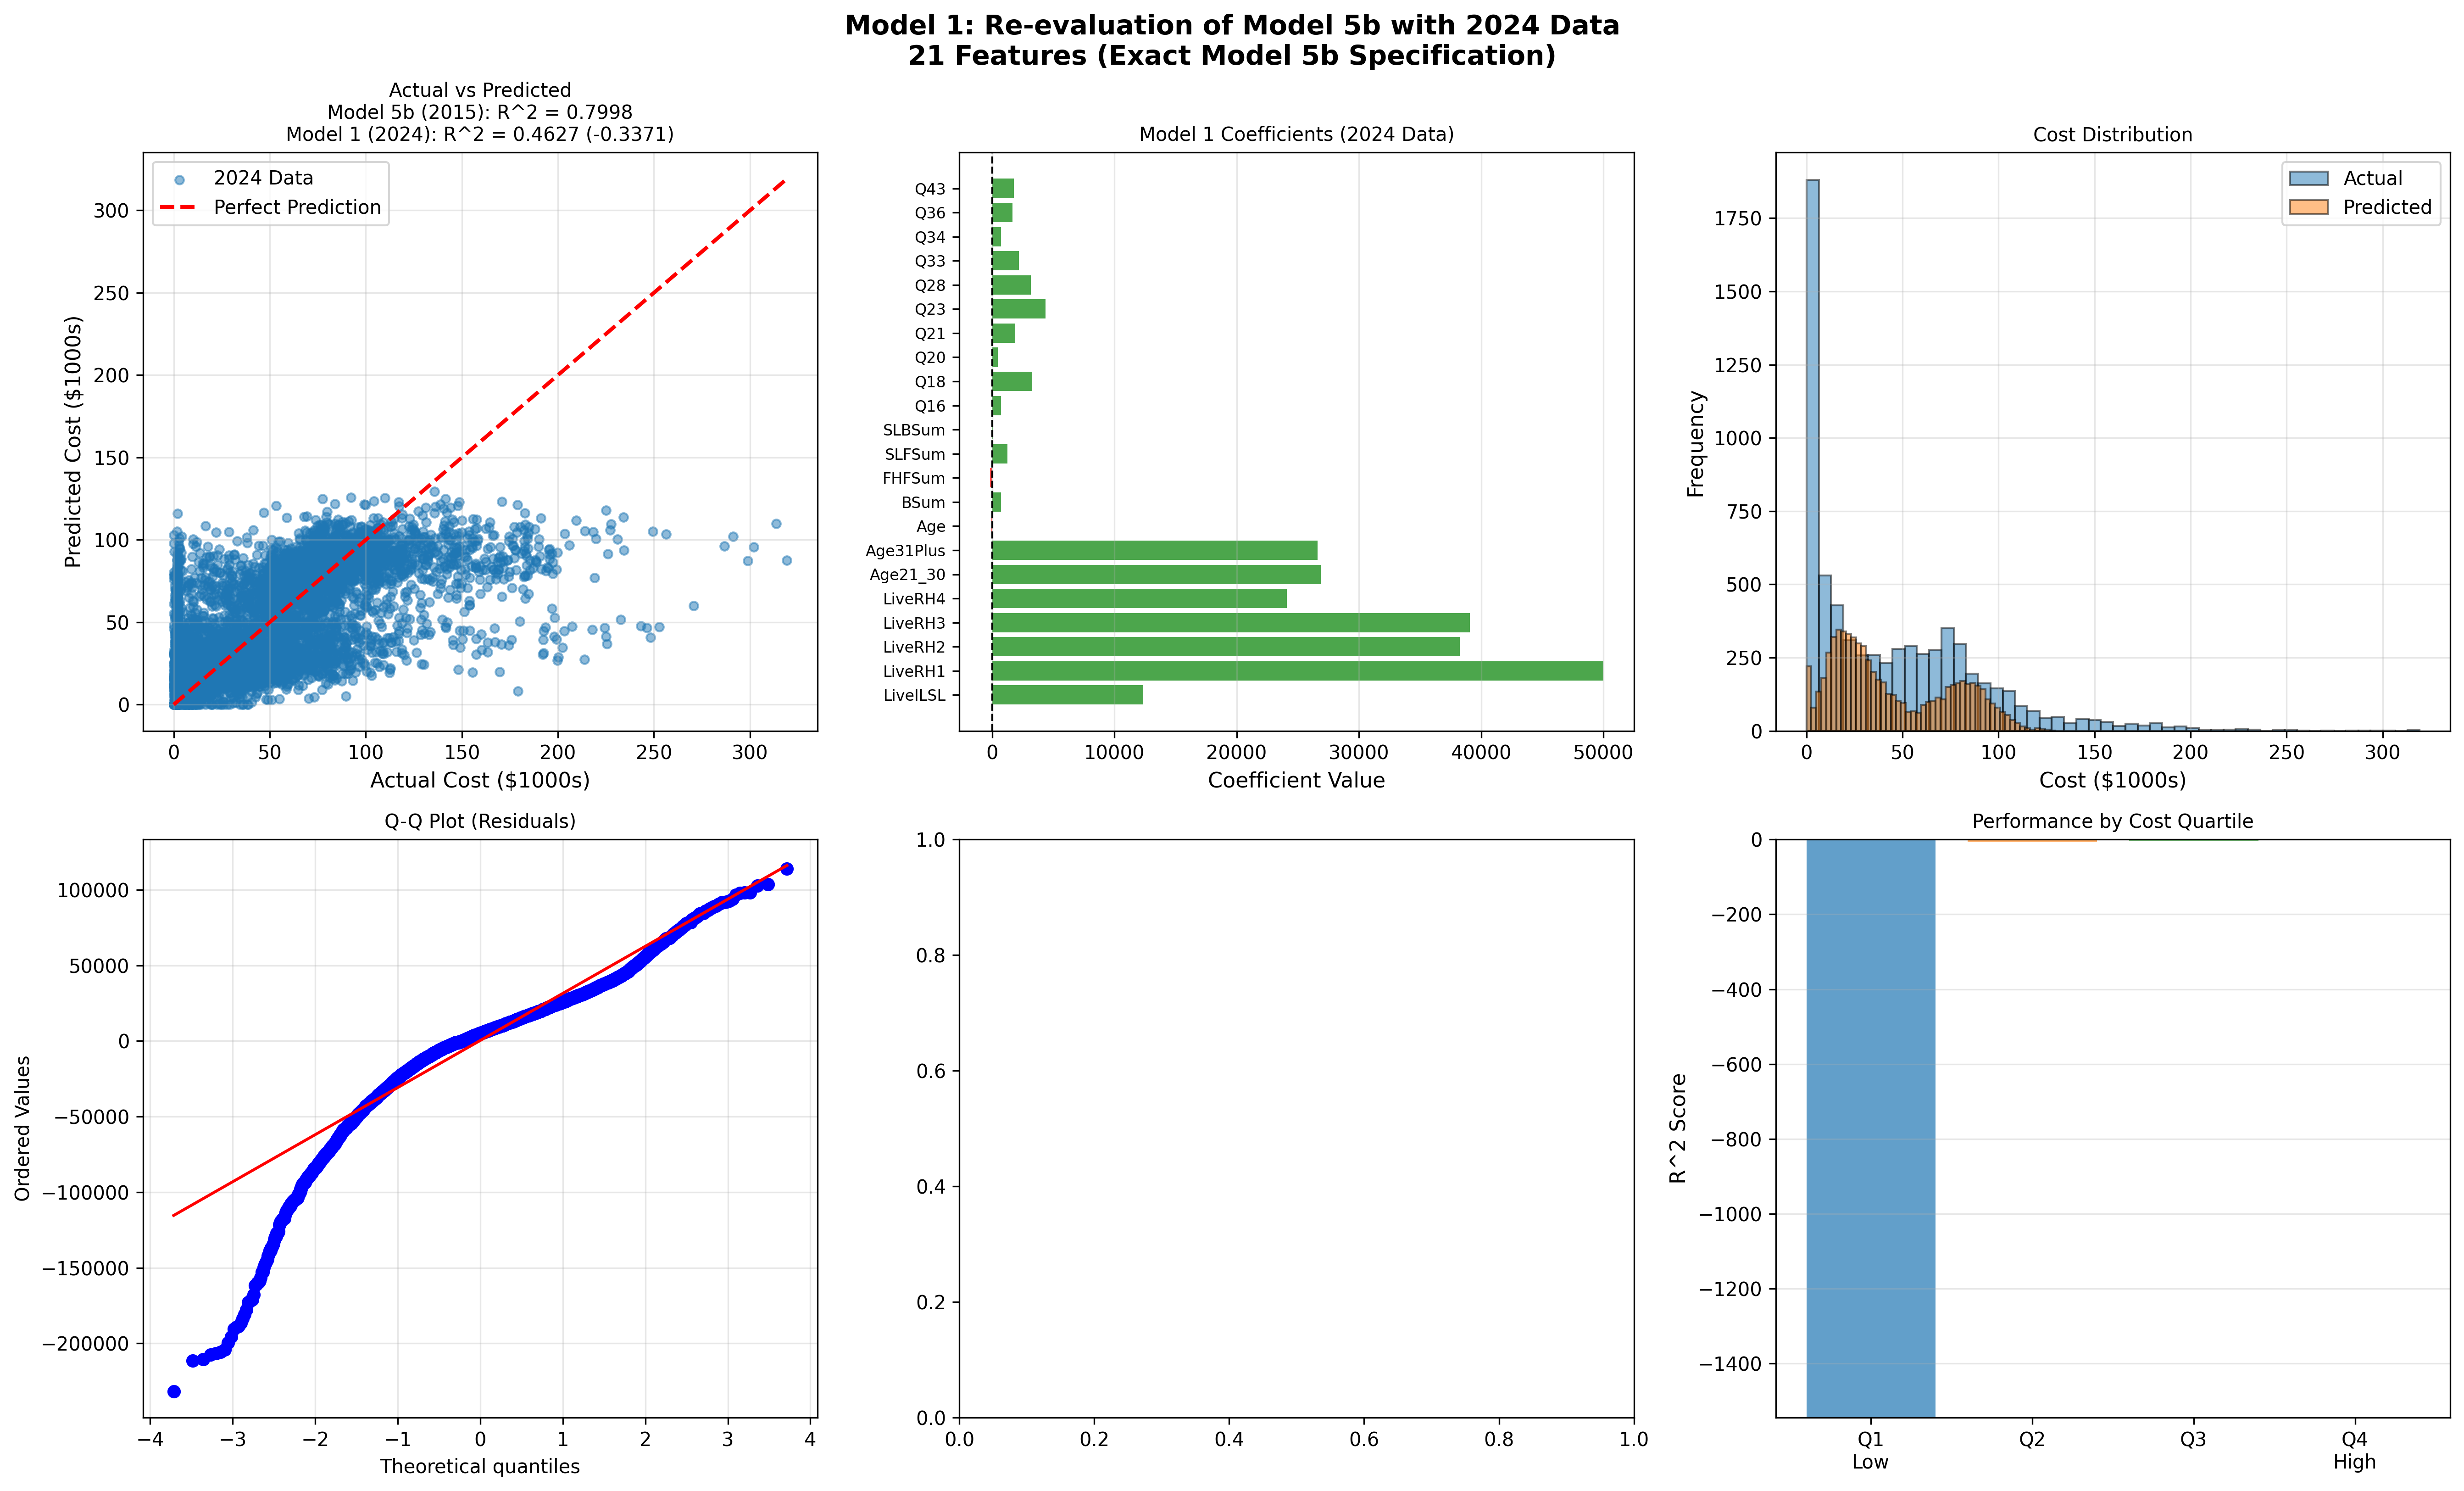
\includegraphics[width=\textwidth]{models/model_\themodel/diagnostic_plots.png}
    \caption{Model Diagnostic Plots --- Shows actual vs.\ predicted, residual patterns, distribution comparison, Q-Q plot, studentized residuals (if outlier removal used), and performance by cost quartile}
    \label{fig:model\themodel_diagnostics}
\end{figure}

\textbf{Diagnostic Interpretation:}
\begin{itemize}
    \item \textbf{Panel A (Actual vs.\ Predicted)}: Points should cluster along the 45° line. Systematic deviations indicate bias in certain cost ranges.
    \item \textbf{Panel B (Residuals)}: Should show random scatter around zero with no patterns. Funnel shapes indicate heteroscedasticity.
    \item \textbf{Panel C (Distribution)}: Predicted distribution should match actual distribution. Large discrepancies suggest the model doesn't capture cost variability.
    \item \textbf{Panel D (Q-Q Plot)}: Tests normality of residuals. Points should follow the diagonal line. Deviations at tails indicate non-normality.
    \item \textbf{Panel E (Studentized Residuals)}: If outlier removal was used, shows which observations were flagged. Should see most points within threshold bounds.
    \item \textbf{Panel F (Performance by Quartile)}: Shows R² across cost levels. Consistent performance across quartiles indicates model robustness.
\end{itemize}

% ============================================
% END OF UNIVERSAL TEMPLATE
% Model-specific content should be added after this point
% ============================================
%
% Now all \M... commands in the template will use Model 1's values
% ============================================
\newcommand{\SetupModelTemplate}[1]{%
    % #1 = Model word (One, Two, Three, ..., Ten)
    
    % ===== Performance Metrics =====
    \expandafter\def\csname MRSquaredTrain\endcsname{\csname Model#1RSquaredTrain\endcsname}%
    \expandafter\def\csname MRSquaredTest\endcsname{\csname Model#1RSquaredTest\endcsname}%
    \expandafter\def\csname MRMSETrain\endcsname{\csname Model#1RMSETrain\endcsname}%
    \expandafter\def\csname MRMSETest\endcsname{\csname Model#1RMSETest\endcsname}%
    \expandafter\def\csname MRMSETrainSqrt\endcsname{\csname Model#1RMSETrainSqrt\endcsname}%
    \expandafter\def\csname MRMSETestSqrt\endcsname{\csname Model#1RMSETestSqrt\endcsname}%    
    \expandafter\def\csname MMAETrain\endcsname{\csname Model#1MAETrain\endcsname}%
    \expandafter\def\csname MMAETest\endcsname{\csname Model#1MAETest\endcsname}%
    \expandafter\def\csname MMAPETrain\endcsname{\csname Model#1MAPETrain\endcsname}%
    \expandafter\def\csname MMAPETest\endcsname{\csname Model#1MAPETest\endcsname}%
    \expandafter\def\csname MCVMean\endcsname{\csname Model#1CVMean\endcsname}%
    \expandafter\def\csname MCVStd\endcsname{\csname Model#1CVStd\endcsname}%
    \expandafter\def\csname MTrainingSamples\endcsname{\csname Model#1TrainingSamples\endcsname}%
    \expandafter\def\csname MTestSamples\endcsname{\csname Model#1TestSamples\endcsname}%
    
    % ===== Accuracy Bands =====
    \expandafter\def\csname MWithinOneK\endcsname{\csname Model#1WithinOneK\endcsname}%
    \expandafter\def\csname MWithinTwoK\endcsname{\csname Model#1WithinTwoK\endcsname}%
    \expandafter\def\csname MWithinFiveK\endcsname{\csname Model#1WithinFiveK\endcsname}%
    \expandafter\def\csname MWithinTenK\endcsname{\csname Model#1WithinTenK\endcsname}%
    \expandafter\def\csname MWithinTwentyK\endcsname{\csname Model#1WithinTwentyK\endcsname}%
    
    % ===== Variance Metrics =====
    \expandafter\def\csname MCVActual\endcsname{\csname Model#1CVActual\endcsname}%
    \expandafter\def\csname MCVPredicted\endcsname{\csname Model#1CVPredicted\endcsname}%
    \expandafter\def\csname MPredictionInterval\endcsname{\csname Model#1PredictionInterval\endcsname}%
    \expandafter\def\csname MBudgetActualCorr\endcsname{\csname Model#1BudgetActualCorr\endcsname}%
    
    % ===== Outlier Metrics =====
    \expandafter\def\csname MOutliersRemoved\endcsname{\csname Model#1OutliersRemoved\endcsname}%
    \expandafter\def\csname MOutlierPct\endcsname{\csname Model#1OutlierPct\endcsname}%
    
    % ===== Subgroup Metrics - Living Settings =====
    \expandafter\def\csname MSubgroupLivingFHRSquared\endcsname{\csname Model#1SubgroupLivingFHRSquared\endcsname}%
    \expandafter\def\csname MSubgroupLivingFHRMSE\endcsname{\csname Model#1SubgroupLivingFHRMSE\endcsname}%
    \expandafter\def\csname MSubgroupLivingFHBias\endcsname{\csname Model#1SubgroupLivingFHBias\endcsname}%
    \expandafter\def\csname MSubgroupLivingFHN\endcsname{\csname Model#1SubgroupLivingFHN\endcsname}%
    
    \expandafter\def\csname MSubgroupLivingILSLRSquared\endcsname{\csname Model#1SubgroupLivingILSLRSquared\endcsname}%
    \expandafter\def\csname MSubgroupLivingILSLRMSE\endcsname{\csname Model#1SubgroupLivingILSLRMSE\endcsname}%
    \expandafter\def\csname MSubgroupLivingILSLBias\endcsname{\csname Model#1SubgroupLivingILSLBias\endcsname}%
    \expandafter\def\csname MSubgroupLivingILSLN\endcsname{\csname Model#1SubgroupLivingILSLN\endcsname}%
    
    \expandafter\def\csname MSubgroupLivingRHOneFourRSquared\endcsname{\csname Model#1SubgroupLivingRHOneFourRSquared\endcsname}%
    \expandafter\def\csname MSubgroupLivingRHOneFourRMSE\endcsname{\csname Model#1SubgroupLivingRHOneFourRMSE\endcsname}%
    \expandafter\def\csname MSubgroupLivingRHOneFourBias\endcsname{\csname Model#1SubgroupLivingRHOneFourBias\endcsname}%
    \expandafter\def\csname MSubgroupLivingRHOneFourN\endcsname{\csname Model#1SubgroupLivingRHOneFourN\endcsname}%
    
    % ===== Subgroup Metrics - Age Groups =====
    \expandafter\def\csname MSubgroupAgeAgeUnderTwentyOneRSquared\endcsname{\csname Model#1SubgroupAgeAgeUnderTwentyOneRSquared\endcsname}%
    \expandafter\def\csname MSubgroupAgeAgeUnderTwentyOneRMSE\endcsname{\csname Model#1SubgroupAgeAgeUnderTwentyOneRMSE\endcsname}%
    \expandafter\def\csname MSubgroupAgeAgeUnderTwentyOneBias\endcsname{\csname Model#1SubgroupAgeAgeUnderTwentyOneBias\endcsname}%
    \expandafter\def\csname MSubgroupAgeAgeUnderTwentyOneN\endcsname{\csname Model#1SubgroupAgeAgeUnderTwentyOneN\endcsname}%
    
    \expandafter\def\csname MSubgroupAgeAgeTwentyOneToThirtyRSquared\endcsname{\csname Model#1SubgroupAgeAgeTwentyOneToThirtyRSquared\endcsname}%
    \expandafter\def\csname MSubgroupAgeAgeTwentyOneToThirtyRMSE\endcsname{\csname Model#1SubgroupAgeAgeTwentyOneToThirtyRMSE\endcsname}%
    \expandafter\def\csname MSubgroupAgeAgeTwentyOneToThirtyBias\endcsname{\csname Model#1SubgroupAgeAgeTwentyOneToThirtyBias\endcsname}%
    \expandafter\def\csname MSubgroupAgeAgeTwentyOneToThirtyN\endcsname{\csname Model#1SubgroupAgeAgeTwentyOneToThirtyN\endcsname}%
    
    \expandafter\def\csname MSubgroupAgeAgeThirtyOnePlusRSquared\endcsname{\csname Model#1SubgroupAgeAgeThirtyOnePlusRSquared\endcsname}%
    \expandafter\def\csname MSubgroupAgeAgeThirtyOnePlusRMSE\endcsname{\csname Model#1SubgroupAgeAgeThirtyOnePlusRMSE\endcsname}%
    \expandafter\def\csname MSubgroupAgeAgeThirtyOnePlusBias\endcsname{\csname Model#1SubgroupAgeAgeThirtyOnePlusBias\endcsname}%
    \expandafter\def\csname MSubgroupAgeAgeThirtyOnePlusN\endcsname{\csname Model#1SubgroupAgeAgeThirtyOnePlusN\endcsname}%
    
    % ===== Subgroup Metrics - Cost Quartiles =====
    \expandafter\def\csname MSubgroupCostQOneLowRSquared\endcsname{\csname Model#1SubgroupCostQOneLowRSquared\endcsname}%
    \expandafter\def\csname MSubgroupCostQOneLowRMSE\endcsname{\csname Model#1SubgroupCostQOneLowRMSE\endcsname}%
    \expandafter\def\csname MSubgroupCostQOneLowBias\endcsname{\csname Model#1SubgroupCostQOneLowBias\endcsname}%
    \expandafter\def\csname MSubgroupCostQOneLowN\endcsname{\csname Model#1SubgroupCostQOneLowN\endcsname}%
    
    \expandafter\def\csname MSubgroupCostQTwoRSquared\endcsname{\csname Model#1SubgroupCostQTwoRSquared\endcsname}%
    \expandafter\def\csname MSubgroupCostQTwoRMSE\endcsname{\csname Model#1SubgroupCostQTwoRMSE\endcsname}%
    \expandafter\def\csname MSubgroupCostQTwoBias\endcsname{\csname Model#1SubgroupCostQTwoBias\endcsname}%
    \expandafter\def\csname MSubgroupCostQTwoN\endcsname{\csname Model#1SubgroupCostQTwoN\endcsname}%
    
    \expandafter\def\csname MSubgroupCostQThreeRSquared\endcsname{\csname Model#1SubgroupCostQThreeRSquared\endcsname}%
    \expandafter\def\csname MSubgroupCostQThreeRMSE\endcsname{\csname Model#1SubgroupCostQThreeRMSE\endcsname}%
    \expandafter\def\csname MSubgroupCostQThreeBias\endcsname{\csname Model#1SubgroupCostQThreeBias\endcsname}%
    \expandafter\def\csname MSubgroupCostQThreeN\endcsname{\csname Model#1SubgroupCostQThreeN\endcsname}%
    
    \expandafter\def\csname MSubgroupCostQFourHighRSquared\endcsname{\csname Model#1SubgroupCostQFourHighRSquared\endcsname}%
    \expandafter\def\csname MSubgroupCostQFourHighRMSE\endcsname{\csname Model#1SubgroupCostQFourHighRMSE\endcsname}%
    \expandafter\def\csname MSubgroupCostQFourHighBias\endcsname{\csname Model#1SubgroupCostQFourHighBias\endcsname}%
    \expandafter\def\csname MSubgroupCostQFourHighN\endcsname{\csname Model#1SubgroupCostQFourHighN\endcsname}%
    
    % ===== Population Scenarios =====
    % Current Baseline
    \expandafter\def\csname MPopcurrentbaselineClients\endcsname{\csname Model#1PopcurrentbaselineClients\endcsname}%
    \expandafter\def\csname MPopcurrentbaselineAvgAlloc\endcsname{\csname Model#1PopcurrentbaselineAvgAlloc\endcsname}%
    \expandafter\def\csname MPopcurrentbaselineWaitlistChange\endcsname{\csname Model#1PopcurrentbaselineWaitlistChange\endcsname}%
    \expandafter\def\csname MPopcurrentbaselineWaitlistPct\endcsname{\csname Model#1PopcurrentbaselineWaitlistPct\endcsname}%
    
    % Model Balanced
    \expandafter\def\csname MPopmodelbalancedClients\endcsname{\csname Model#1PopmodelbalancedClients\endcsname}%
    \expandafter\def\csname MPopmodelbalancedAvgAlloc\endcsname{\csname Model#1PopmodelbalancedAvgAlloc\endcsname}%
    \expandafter\def\csname MPopmodelbalancedWaitlistChange\endcsname{\csname Model#1PopmodelbalancedWaitlistChange\endcsname}%
    \expandafter\def\csname MPopmodelbalancedWaitlistPct\endcsname{\csname Model#1PopmodelbalancedWaitlistPct\endcsname}%
    
    % Model Efficiency
    \expandafter\def\csname MPopmodelefficiencyClients\endcsname{\csname Model#1PopmodelefficiencyClients\endcsname}%
    \expandafter\def\csname MPopmodelefficiencyAvgAlloc\endcsname{\csname Model#1PopmodelefficiencyAvgAlloc\endcsname}%
    \expandafter\def\csname MPopmodelefficiencyWaitlistChange\endcsname{\csname Model#1PopmodelefficiencyWaitlistChange\endcsname}%
    \expandafter\def\csname MPopmodelefficiencyWaitlistPct\endcsname{\csname Model#1PopmodelefficiencyWaitlistPct\endcsname}%
    
    % Category Focused
    \expandafter\def\csname MPopcategoryfocusedClients\endcsname{\csname Model#1PopcategoryfocusedClients\endcsname}%
    \expandafter\def\csname MPopcategoryfocusedAvgAlloc\endcsname{\csname Model#1PopcategoryfocusedAvgAlloc\endcsname}%
    \expandafter\def\csname MPopcategoryfocusedWaitlistChange\endcsname{\csname Model#1PopcategoryfocusedWaitlistChange\endcsname}%
    \expandafter\def\csname MPopcategoryfocusedWaitlistPct\endcsname{\csname Model#1PopcategoryfocusedWaitlistPct\endcsname}%
}



%\usepackage[fontsize=10pt]{scrextend} 
%\setmargins{2.5cm}{2.5cm}{15cm}{23cm}{14pt}{3cm}{0pt}{2cm}
% \setmargins{3.5cm}%			% left edge
% 		   {2.5cm}%     % top edge
%            {14.7cm}%		% text width
%            {21.42cm}%   % text hight
%            {14pt}%			% header hight
%            {3cm}%   	  % header distance
%            {0pt}%				% footer hight
%            {2cm}%    	  % footer distance         

%\usepackage{t1enc} % as usual
%\usepackage[latin1]{inputenc} % as usual
%\usepackage{times}		
%\usepackage{mathptmx}  	%mathematical fonts for use with times, I encountered some problems using this package togather with pdftex, which I was not able to resolve

% ********* Graphics definition *******
%\usepackage[pdftex]{graphicx} % required to import graphic files
\usepackage{color} %allows to mark some entries in the tables with color
\usepackage[pdftex]{graphicx}
\usepackage{tcolorbox}
\usepackage{eso-pic} % these two are required to add the little picture on top of every page
\usepackage{everyshi} % these two are required to add the little picture on top of every page
\renewcommand{\floatpagefraction}{0.7} %default:0.5 allows two big pictures on one page

%********** Enabling landscape orientation *******
\usepackage{rotating}

\usepackage{draftwatermark}
\SetWatermarkText{\phantom{} \\DRAFT}
\SetWatermarkScale{4} % Adjust size
\SetWatermarkColor[gray]{0.9} % Set color and transparency

%********** Enybeling Hyperlinks *******
\usepackage[pdfborder=000,pdftex=true]{hyperref}% this enables jumping from a reference and table of content in the pdf file to its target

% ********* Table layout **************
\usepackage{booktabs}	  	%design of table, has an excellent documentation
%\usepackage{lscape}			%use this if you want to rotate the table together with the lines around the table

% ********* Caption Layout ************
\usepackage{ccaption} % allows special formating of the captions
\captionnamefont{\footnotesize\sffamily} % defines the font of the caption name (e.g. Figure: or Table:)
\captiontitlefont{\footnotesize\sffamily} % defines the font of the caption text (same as above, but not bold)
\setlength{\abovecaptionskip}{0mm} %lowers the distace of captions to the figure

\usepackage{sidecap}
\usepackage{tikz}
\usetikzlibrary{decorations.pathreplacing}

% ********* Header and Footer **********
% This is something to play with forever. I use here the advanced settings of the KOMA script
%\usepackage{scrlayer-scrpage} %scrpage2} %header and footer using the options for the KOMA script
%\renewcommand{\headfont}{\footnotesize\sffamily} % font for the header
%\renewcommand{\pnumfont}{\footnotesize\sffamily} % font for the pagenumbers

%the following lines define the pagestyle for the main document
% \defpagestyle{cb}{%
% (\textwidth,0pt)% sets the border line above the header
% {\pagemark\hfill\headmark\hfill}% doublesided, left page
% {\hfill\headmark\hfill\pagemark}% doublesided, right page
% {\hfill\headmark\hfill\pagemark}%  onesided
% (\textwidth,1pt)}% sets the border line below the header
% %
% {(\textwidth,1pt)% sets the border line above the footer
% {\scshape Preliminary report \hfill Correlates of Student Success 2020}% doublesided, left page
% {\scshape Correlates of Student Success 2020 \hfill Preliminary report}% doublesided, right page
% {\scshape Correlates of Student Success 2020 \hfill Preliminary report} % one sided printing
% (\textwidth,0pt)% sets the border line below the footer
% }

% %this defines the page style for the first pages: all empty
% \renewpagestyle{plain}%
% 	{(\textwidth,0pt)%
% 		{\hfill}{\hfill}{\hfill}%
% 	(\textwidth,0pt)}%
% 	{(\textwidth,0pt)%	
% 		{\hfill}{\hfill}{\hfill}%
% 	(\textwidth,0pt)}

%********** Footnotes **********
\renewcommand{\footnoterule}{\rule{5cm}{0.2mm} \vspace{0.3cm}} %increases the distance of footnotes from the text
%\deffootnote[1em]{1em}{1em}{\textsuperscript{\normalfont\thefootnotemark}} %some more formattion on footnotes

%Make section number before figure number.
\renewcommand{\thefigure}{\thesection-\arabic{figure}}

% Display subsections in the TOC
\setcounter{tocdepth}{3}
\setcounter{secnumdepth}{3}

%################ End Preferences #####################

%********** Begin Frontmatter **********

\pagestyle{plain} % on headers or footers on the first page

%########################### MACROS #################################


\usepackage{fancyhdr} % this is for headers and footers
\usepackage[pages=some]{background}
%\backgroundsetup{
%scale=1.0,color=black,opacity=1,angle=0,
%contents={
%  \includegraphics[width=1.25\paperwidth,height=1.3\paperheight]{../figures/cover/BackgroundCover}
%  }
%}
\backgroundsetup{
scale=1.0,color=black,opacity=1,angle=0,
contents={
  \includegraphics[width=0.5\paperwidth,height=0.5\paperheight]{../figures/cover/BackgroundCover}
  }
}
%%************************************************
\pagestyle{fancyplain}
\fancyhf{}
\lhead{
\includegraphics[width=1cm]{../assets/ISF-logo-tight.png}} % 
\rhead{\footnotesize{\sc{iBudget - Information Systems of Florida}}} 
\setcounter{page}{1} 
\lfoot{Obsolescence date: 10/15/2025}%\today -
%\cfoot{\sc{\footnotesize }}
\rfoot{Page \thepage \hspace{0.005cm} of \pageref*{TotPages}} % \ThePageCount
%%************************************************

%\hypersetup{colorlinks=true, linkcolor=blue, filecolor=blue, pagecolor=blue, urlcolor=blue}
%Text styles
\definecolor{Input}{rgb}{0.0,0.45,0.0} % a dark green
\definecolor{Output}{rgb}{0.0,0.0,1.0} % blue
\definecolor{SrcBckgrnd}{rgb}{0.95,0.95,0.95} % blue
\definecolor{HW}{rgb}{0.8,0.0,0.0} % red
\definecolor{UTSABlue}{rgb}{0.047,0.137,0.251} 
\definecolor{UTSAOrange}{rgb}{0.945,0.353,0.133} 
\newcommand\textstyleInput[1]{\texttt{\textbf{\textcolor[rgb]{0.0,0.45,0.0}{#1}}}}
\newcommand\textstyleOutput[1]{\texttt{{\textcolor[rgb]{0.0,0.75,0.0}{#1}}}} 

\newcommand{\low}{\textnormal{\tiny\textit{low}}\hspace{-5pt}}
\newcommand{\high}{\textnormal{\tiny \textit{high}}\hspace{-5pt}}
\newcommand{\vv}{{\bf v}}
\newcommand{\mb}{\left[\begin{matrix}}
\newcommand{\me}{\end{matrix}\right]}
\newcommand{\lam}{\lambda}
\newcommand{\PP}{\hbox{I\kern-0.2em\hbox{P}}}
\newcommand{\RR}{\hbox{I\kern-0.2em\hbox{R}}}
\newcommand{\ZZ}{\hbox{Z\kern-0.35em\hbox{Z}}}
\newcommand{\R}{{\mathbb{R}}}
\newcommand{\N}{{\mathbb{N}}}
\newcommand{\Z}{{\mathbb{Z}}}
\newcommand{\Q}{{\mathbb{Q}}}
\newcommand{\C}{{\mathbb{C}}}
\newcommand{\M}{{\mathbb{M}}}
\newcommand{\e}{\mathrm{e}}
\newcommand{\ee}{\mathrm{e}}
\newcommand{\mat}[1]{\bmatrix #1\endbmatrix}
\newcommand{\sinc}{\operatorname{sinc}}
\newcommand{\rect}{\operatorname{rect}}
\newcommand{\conj}{\overline}
\newcommand{\ebb}{\mathrm{\textbf{e}}}
\newcommand{\mbb}{\textbf{m}}
\newcommand{\y}{\textbf{y}}
\newcommand{\x}{\textbf{x}}
\newcommand{\X}{\textbf{X}}
\newcommand{\z}{\textbf{z}}
\newcommand{\A}{\textbf{A}}
\newcommand{\Sbb}{\textbf{S}}
\newcommand\bb{\textbf{b}}
\newcommand\vs{\vspace{0.2in}}
%\newcommand{\vs}{\vspace*{0.1in}\noindent}

% Define commands for the symbols with tikz
% \newcommand{\greencheck}{%
%     \tikz\fill[scale=0.4,color=green!70!black](0,.35) -- (.25,0) -- (1,.7) -- (.25,.15) -- cycle;%
% }
% \newcommand{\yellowwarning}{%
%     \tikz\draw[scale=0.4,color=yellow!80!orange,fill=yellow!80!orange] (0,0) -- (1,0) -- (0.5,0.866) -- cycle;%
%     \tikz\node[scale=0.3] at (0.2,0.15) {\textbf{!}};%
% }
% \newcommand{\redcross}{%
%     \tikz[scale=0.4]{
%         \draw[color=red,line width=1pt] (0,0) -- (1,1);
%         \draw[color=red,line width=1pt] (0,1) -- (1,0);
%     }%
% }

% Define commands for the symbols with fontawsome
\newcommand{\greencheck}{\textcolor{green!70!black}{\faCheckCircle}\hspace{0.05in}}
\newcommand{\yellowwarning}{\textcolor{yellow!80!orange}{\faExclamationTriangle}\hspace{0.05in}}
\newcommand{\redcross}{\textcolor{red}{\faTimesCircle}\hspace{0.05in}}

\newcounter{example}[section]
\newenvironment{example}[1][]{\refstepcounter{example}\par\medskip
   \noindent \textbf{Example~\theexample. #1} \rmfamily}{\medskip}


\newcommand\BeginCode{\medskip\begin{minipage}{0.9\textwidth} \color{Input} \begin{verbatim}} % \vspace{0.1cm}
\newcommand\EndCode{\vspace{0.01cm}\end{minipage}} % \vspace{0.01cm}

\newcommand\s{\color{Input}\ttfamily} % Code snippet. Use: {\s code here}

\newcounter{QaA}
\newenvironment{EQA}[1][]{\refstepcounter{QaA} \color{HW} Record your explanation as answer \#\theQaA. #1 }{\medskip}
\newcommand\QA{\begin{EQA} \end{EQA}} 


% Outlier analysis commands

\newcommand{\WarningRunPiepeline}{WARNING: Value undefined. Run the analysis pipeline}
\newcommand{\placeholder}{\textcolor{red}{[VALUE NOT SET]}}


% Overall statistics
\newcommand{\TheTotalNumberCustomers}{\WarningRunPiepelinee}
\newcommand{\TheInitialYear}{\WarningRunPiepeline}
\newcommand{\TheFinalYear}{\WarningRunPiepeline}
\newcommand{\TheTotalCustomerYears}{\WarningRunPiepeline}

% Customer data availability
\newcommand{\CustomerNumberOneYear}{\WarningRunPiepeline}
\newcommand{\CustomerPctOneYear}{\WarningRunPiepeline}
\newcommand{\CustomerNumberTwoPlusYear}{\WarningRunPiepeline}
\newcommand{\CustomerPctTwoPlusYear}{\WarningRunPiepeline}
\newcommand{\CustomerNumberNoData}{\WarningRunPiepeline}
\newcommand{\CustomerPctNoData}{\WarningRunPiepeline}

% Exclusion statistics
\newcommand{\ExclusionMidYearQSICount}{\WarningRunPiepeline}
\newcommand{\ExclusionMidYearQSIPct}{\WarningRunPiepeline}
\newcommand{\ExclusionLateEntryCount}{\WarningRunPiepeline}
\newcommand{\ExclusionLateEntryPct}{\WarningRunPiepeline}
\newcommand{\ExclusionEarlyExitCount}{\WarningRunPiepeline}
\newcommand{\ExclusionEarlyExitPct}{\WarningRunPiepeline}
\newcommand{\ExclusionNoCostsCount}{\WarningRunPiepeline}
\newcommand{\ExclusionNoCostsPct}{\WarningRunPiepeline}
\newcommand{\ExclusionInsufficientServiceCount}{\WarningRunPiepeline}
\newcommand{\ExclusionInsufficientServicePct}{\WarningRunPiepeline}
\newcommand{\ExclusionNoQSICount}{\WarningRunPiepeline}
\newcommand{\ExclusionNoQSIPct}{\WarningRunPiepeline}

% Cost statistics
\newcommand{\AvgAnnualCost}{\WarningRunPiepeline}
\newcommand{\MedianAnnualCost}{\WarningRunPiepeline}
\newcommand{\StdevAnnualCost}{\WarningRunPiepeline}

% Trajectory analysis
\newcommand{\CustomersWithTrajectory}{\WarningRunPiepeline}
\newcommand{\PctWithTrajectory}{\WarningRunPiepeline}
\newcommand{\CustomersWithGaps}{\WarningRunPiepeline}
\newcommand{\PctWithGaps}{\WarningRunPiepeline}

% Outlier statistics
\newcommand{\OutlierLowerFence}{\WarningRunPiepeline}
\newcommand{\OutlierUpperFence}{\WarningRunPiepeline}
\newcommand{\OutliersBelow}{\WarningRunPiepeline}
\newcommand{\OutliersAbove}{\WarningRunPiepeline}
\newcommand{\OutlierRate}{\WarningRunPiepeline}

% Proration Analysis Commands 

\newcommand{\ProrationFullYearPct}{\WarningRunPipeline}
\newcommand{\ProrationHighCoveragePct}{\WarningRunPipeline}
\newcommand{\ProrationMedianRFull}{\WarningRunPipeline}
\newcommand{\ProrationMedianRLow}{\WarningRunPipeline}
\newcommand{\ProrationTotalCustomerYears}{\WarningRunPipeline}
\newcommand{\ProrationFullYearCount}{\WarningRunPipeline}
\newcommand{\ProrationHighCoverageCount}{\WarningRunPipeline}

% Command definition for all models
\newcommand{\WarningRunPipeline}{\textcolor{red}{[RUN PIPELINE]}}


% Load variable definitions per model

\IfFileExists{models/model_1/model_1_newcommands.tex}{% Model 1 LaTeX Commands (Placeholders)
% Generated: 2025-10-15 16:55:22

\newcommand{\ModelOneRSquaredTrain}{\WarningRunPipeline}
\newcommand{\ModelOneRSquaredTest}{\WarningRunPipeline}
\newcommand{\ModelOneRMSETrain}{\WarningRunPipeline}
\newcommand{\ModelOneRMSETest}{\WarningRunPipeline}
\newcommand{\ModelOneRMSETrainSqrt}{\WarningRunPipeline}
\newcommand{\ModelOneRMSETestSqrt}{\WarningRunPipeline}
\newcommand{\ModelOneMAETrain}{\WarningRunPipeline}
\newcommand{\ModelOneMAETest}{\WarningRunPipeline}
\newcommand{\ModelOneMAPETrain}{\WarningRunPipeline}
\newcommand{\ModelOneMAPETest}{\WarningRunPipeline}
\newcommand{\ModelOneCVMean}{\WarningRunPipeline}
\newcommand{\ModelOneCVStd}{\WarningRunPipeline}
\newcommand{\ModelOneCVCILower}{\WarningRunPipeline}
\newcommand{\ModelOneCVCIUpper}{\WarningRunPipeline}
\newcommand{\ModelOneTrainingSamples}{\WarningRunPipeline}
\newcommand{\ModelOneTestSamples}{\WarningRunPipeline}
\newcommand{\ModelOneWithinOneK}{\WarningRunPipeline}
\newcommand{\ModelOneWithinTwoK}{\WarningRunPipeline}
\newcommand{\ModelOneWithinFiveK}{\WarningRunPipeline}
\newcommand{\ModelOneWithinTenK}{\WarningRunPipeline}
\newcommand{\ModelOneWithinTwentyK}{\WarningRunPipeline}
\newcommand{\ModelOneSubgroupLivingFHN}{\WarningRunPipeline}
\newcommand{\ModelOneSubgroupLivingFHRSquared}{\WarningRunPipeline}
\newcommand{\ModelOneSubgroupLivingFHRMSE}{\WarningRunPipeline}
\newcommand{\ModelOneSubgroupLivingFHBias}{\WarningRunPipeline}
\newcommand{\ModelOneSubgroupLivingILSLN}{\WarningRunPipeline}
\newcommand{\ModelOneSubgroupLivingILSLRSquared}{\WarningRunPipeline}
\newcommand{\ModelOneSubgroupLivingILSLRMSE}{\WarningRunPipeline}
\newcommand{\ModelOneSubgroupLivingILSLBias}{\WarningRunPipeline}
\newcommand{\ModelOneSubgroupLivingRHOneFourN}{\WarningRunPipeline}
\newcommand{\ModelOneSubgroupLivingRHOneFourRSquared}{\WarningRunPipeline}
\newcommand{\ModelOneSubgroupLivingRHOneFourRMSE}{\WarningRunPipeline}
\newcommand{\ModelOneSubgroupLivingRHOneFourBias}{\WarningRunPipeline}
\newcommand{\ModelOneSubgroupAgeAgeUnderTwentyOneN}{\WarningRunPipeline}
\newcommand{\ModelOneSubgroupAgeAgeUnderTwentyOneRSquared}{\WarningRunPipeline}
\newcommand{\ModelOneSubgroupAgeAgeUnderTwentyOneRMSE}{\WarningRunPipeline}
\newcommand{\ModelOneSubgroupAgeAgeUnderTwentyOneBias}{\WarningRunPipeline}
\newcommand{\ModelOneSubgroupAgeAgeTwentyOneToThirtyN}{\WarningRunPipeline}
\newcommand{\ModelOneSubgroupAgeAgeTwentyOneToThirtyRSquared}{\WarningRunPipeline}
\newcommand{\ModelOneSubgroupAgeAgeTwentyOneToThirtyRMSE}{\WarningRunPipeline}
\newcommand{\ModelOneSubgroupAgeAgeTwentyOneToThirtyBias}{\WarningRunPipeline}
\newcommand{\ModelOneSubgroupAgeAgeThirtyOnePlusN}{\WarningRunPipeline}
\newcommand{\ModelOneSubgroupAgeAgeThirtyOnePlusRSquared}{\WarningRunPipeline}
\newcommand{\ModelOneSubgroupAgeAgeThirtyOnePlusRMSE}{\WarningRunPipeline}
\newcommand{\ModelOneSubgroupAgeAgeThirtyOnePlusBias}{\WarningRunPipeline}
\newcommand{\ModelOneSubgroupCostQOneLowN}{\WarningRunPipeline}
\newcommand{\ModelOneSubgroupCostQOneLowRSquared}{\WarningRunPipeline}
\newcommand{\ModelOneSubgroupCostQOneLowRMSE}{\WarningRunPipeline}
\newcommand{\ModelOneSubgroupCostQOneLowBias}{\WarningRunPipeline}
\newcommand{\ModelOneSubgroupCostQTwoN}{\WarningRunPipeline}
\newcommand{\ModelOneSubgroupCostQTwoRSquared}{\WarningRunPipeline}
\newcommand{\ModelOneSubgroupCostQTwoRMSE}{\WarningRunPipeline}
\newcommand{\ModelOneSubgroupCostQTwoBias}{\WarningRunPipeline}
\newcommand{\ModelOneSubgroupCostQThreeN}{\WarningRunPipeline}
\newcommand{\ModelOneSubgroupCostQThreeRSquared}{\WarningRunPipeline}
\newcommand{\ModelOneSubgroupCostQThreeRMSE}{\WarningRunPipeline}
\newcommand{\ModelOneSubgroupCostQThreeBias}{\WarningRunPipeline}
\newcommand{\ModelOneSubgroupCostQFourHighN}{\WarningRunPipeline}
\newcommand{\ModelOneSubgroupCostQFourHighRSquared}{\WarningRunPipeline}
\newcommand{\ModelOneSubgroupCostQFourHighRMSE}{\WarningRunPipeline}
\newcommand{\ModelOneSubgroupCostQFourHighBias}{\WarningRunPipeline}
\newcommand{\ModelOneCVActual}{\WarningRunPipeline}
\newcommand{\ModelOneCVPredicted}{\WarningRunPipeline}
\newcommand{\ModelOnePredictionInterval}{\WarningRunPipeline}
\newcommand{\ModelOneBudgetActualCorr}{\WarningRunPipeline}
\newcommand{\ModelOnePopcurrentbaselineClients}{\WarningRunPipeline}
\newcommand{\ModelOnePopcurrentbaselineAvgAlloc}{\WarningRunPipeline}
\newcommand{\ModelOnePopcurrentbaselineWaitlistChange}{\WarningRunPipeline}
\newcommand{\ModelOnePopcurrentbaselineWaitlistPct}{\WarningRunPipeline}
\newcommand{\ModelOnePopmodelbalancedClients}{\WarningRunPipeline}
\newcommand{\ModelOnePopmodelbalancedAvgAlloc}{\WarningRunPipeline}
\newcommand{\ModelOnePopmodelbalancedWaitlistChange}{\WarningRunPipeline}
\newcommand{\ModelOnePopmodelbalancedWaitlistPct}{\WarningRunPipeline}
\newcommand{\ModelOnePopmodelefficiencyClients}{\WarningRunPipeline}
\newcommand{\ModelOnePopmodelefficiencyAvgAlloc}{\WarningRunPipeline}
\newcommand{\ModelOnePopmodelefficiencyWaitlistChange}{\WarningRunPipeline}
\newcommand{\ModelOnePopmodelefficiencyWaitlistPct}{\WarningRunPipeline}
\newcommand{\ModelOnePopcategoryfocusedClients}{\WarningRunPipeline}
\newcommand{\ModelOnePopcategoryfocusedAvgAlloc}{\WarningRunPipeline}
\newcommand{\ModelOnePopcategoryfocusedWaitlistChange}{\WarningRunPipeline}
\newcommand{\ModelOnePopcategoryfocusedWaitlistPct}{\WarningRunPipeline}
\newcommand{\ModelOneStudentizedResidualsMean}{\WarningRunPipeline}
\newcommand{\ModelOneStudentizedResidualsStd}{\WarningRunPipeline}
\newcommand{\ModelOnePctWithinThreshold}{\WarningRunPipeline}
\newcommand{\ModelOneOutliersRemoved}{\WarningRunPipeline}
\newcommand{\ModelOneOutlierPct}{\WarningRunPipeline}
\newcommand{\ModelOneNumFeatures}{\WarningRunPipeline}

% Model 5b Comparison Commands
\newcommand{\ModelOneFiveBRSquaredTwoThousandFifteen}{\WarningRunPipeline}
\newcommand{\ModelOneFiveBSBCTwoThousandFifteen}{\WarningRunPipeline}
\newcommand{\ModelOneFiveBRMSETwoThousandFifteen}{\WarningRunPipeline}
\newcommand{\ModelOneFiveBOutlierPctTwoThousandFifteen}{\WarningRunPipeline}
\newcommand{\ModelOneRSquaredDeltaFromTwoThousandFifteen}{\WarningRunPipeline}
\newcommand{\ModelOneSBC}{\WarningRunPipeline}
\newcommand{\ModelOneSBCDeltaFromTwoThousandFifteen}{\WarningRunPipeline}
\newcommand{\ModelOneOutlierPctDeltaFromTwoThousandFifteen}{\WarningRunPipeline}
\newcommand{\ModelOneRMSEDeltaFromTwoThousandFifteen}{\WarningRunPipeline}
}{}
\IfFileExists{models/model_2/model_2_newcommands.tex}{% Model 2 Command Definitions
% Generated: 2025-09-29 23:34:36.724569

\newcommand{\ModelTwoRSquaredTrain}{\WarningRunPipeline}
\newcommand{\ModelTwoRSquaredTest}{\WarningRunPipeline}
\newcommand{\ModelTwoRMSETrain}{\WarningRunPipeline}
\newcommand{\ModelTwoRMSETest}{\WarningRunPipeline}
\newcommand{\ModelTwoMAETrain}{\WarningRunPipeline}
\newcommand{\ModelTwoMAETest}{\WarningRunPipeline}
\newcommand{\ModelTwoMAPETrain}{\WarningRunPipeline}
\newcommand{\ModelTwoMAPETest}{\WarningRunPipeline}
\newcommand{\ModelTwoCVMean}{\WarningRunPipeline}
\newcommand{\ModelTwoCVStd}{\WarningRunPipeline}
\newcommand{\ModelTwoWithinFiveK}{\WarningRunPipeline}
\newcommand{\ModelTwoWithinTenK}{\WarningRunPipeline}
\newcommand{\ModelTwoWithinTwentyK}{\WarningRunPipeline}
\newcommand{\ModelTwoTrainingSamples}{\WarningRunPipeline}
\newcommand{\ModelTwoTestSamples}{\WarningRunPipeline}

% GLM-Specific Commands
\newcommand{\ModelTwoDispersion}{\WarningRunPipeline}
\newcommand{\ModelTwoDevianceRSquared}{\WarningRunPipeline}
\newcommand{\ModelTwoMcFaddenRSquared}{\WarningRunPipeline}
\newcommand{\ModelTwoAIC}{\WarningRunPipeline}
\newcommand{\ModelTwoBIC}{\WarningRunPipeline}
\newcommand{\ModelTwoParameters}{\WarningRunPipeline}
}{}
\IfFileExists{models/model_3/model_3_newcommands.tex}{% Model 3 LaTeX Commands (Placeholders)
% Generated: 2025-10-12 14:57:42

\newcommand{\ModelThreeRSquaredTrain}{\WarningRunPipeline}
\newcommand{\ModelThreeRSquaredTest}{\WarningRunPipeline}
\newcommand{\ModelThreeRMSETrain}{\WarningRunPipeline}
\newcommand{\ModelThreeRMSETest}{\WarningRunPipeline}
\newcommand{\ModelThreeRMSETrainSqrt}{\WarningRunPipeline}
\newcommand{\ModelThreeRMSETestSqrt}{\WarningRunPipeline}
\newcommand{\ModelThreeMAETrain}{\WarningRunPipeline}
\newcommand{\ModelThreeMAETest}{\WarningRunPipeline}
\newcommand{\ModelThreeMAPETrain}{\WarningRunPipeline}
\newcommand{\ModelThreeMAPETest}{\WarningRunPipeline}
\newcommand{\ModelThreeCVMean}{\WarningRunPipeline}
\newcommand{\ModelThreeCVStd}{\WarningRunPipeline}
\newcommand{\ModelThreeCVCILower}{\WarningRunPipeline}
\newcommand{\ModelThreeCVCIUpper}{\WarningRunPipeline}
\newcommand{\ModelThreeTrainingSamples}{\WarningRunPipeline}
\newcommand{\ModelThreeTestSamples}{\WarningRunPipeline}
\newcommand{\ModelThreeWithinOneK}{\WarningRunPipeline}
\newcommand{\ModelThreeWithinTwoK}{\WarningRunPipeline}
\newcommand{\ModelThreeWithinFiveK}{\WarningRunPipeline}
\newcommand{\ModelThreeWithinTenK}{\WarningRunPipeline}
\newcommand{\ModelThreeWithinTwentyK}{\WarningRunPipeline}
\newcommand{\ModelThreeSubgroupLivingFHN}{\WarningRunPipeline}
\newcommand{\ModelThreeSubgroupLivingFHRSquared}{\WarningRunPipeline}
\newcommand{\ModelThreeSubgroupLivingFHRMSE}{\WarningRunPipeline}
\newcommand{\ModelThreeSubgroupLivingFHBias}{\WarningRunPipeline}
\newcommand{\ModelThreeSubgroupLivingILSLN}{\WarningRunPipeline}
\newcommand{\ModelThreeSubgroupLivingILSLRSquared}{\WarningRunPipeline}
\newcommand{\ModelThreeSubgroupLivingILSLRMSE}{\WarningRunPipeline}
\newcommand{\ModelThreeSubgroupLivingILSLBias}{\WarningRunPipeline}
\newcommand{\ModelThreeSubgroupLivingRHOneFourN}{\WarningRunPipeline}
\newcommand{\ModelThreeSubgroupLivingRHOneFourRSquared}{\WarningRunPipeline}
\newcommand{\ModelThreeSubgroupLivingRHOneFourRMSE}{\WarningRunPipeline}
\newcommand{\ModelThreeSubgroupLivingRHOneFourBias}{\WarningRunPipeline}
\newcommand{\ModelThreeSubgroupAgeAgeUnderTwentyOneN}{\WarningRunPipeline}
\newcommand{\ModelThreeSubgroupAgeAgeUnderTwentyOneRSquared}{\WarningRunPipeline}
\newcommand{\ModelThreeSubgroupAgeAgeUnderTwentyOneRMSE}{\WarningRunPipeline}
\newcommand{\ModelThreeSubgroupAgeAgeUnderTwentyOneBias}{\WarningRunPipeline}
\newcommand{\ModelThreeSubgroupAgeAgeTwentyOneToThirtyN}{\WarningRunPipeline}
\newcommand{\ModelThreeSubgroupAgeAgeTwentyOneToThirtyRSquared}{\WarningRunPipeline}
\newcommand{\ModelThreeSubgroupAgeAgeTwentyOneToThirtyRMSE}{\WarningRunPipeline}
\newcommand{\ModelThreeSubgroupAgeAgeTwentyOneToThirtyBias}{\WarningRunPipeline}
\newcommand{\ModelThreeSubgroupAgeAgeThirtyOnePlusN}{\WarningRunPipeline}
\newcommand{\ModelThreeSubgroupAgeAgeThirtyOnePlusRSquared}{\WarningRunPipeline}
\newcommand{\ModelThreeSubgroupAgeAgeThirtyOnePlusRMSE}{\WarningRunPipeline}
\newcommand{\ModelThreeSubgroupAgeAgeThirtyOnePlusBias}{\WarningRunPipeline}
\newcommand{\ModelThreeSubgroupCostQOneLowN}{\WarningRunPipeline}
\newcommand{\ModelThreeSubgroupCostQOneLowRSquared}{\WarningRunPipeline}
\newcommand{\ModelThreeSubgroupCostQOneLowRMSE}{\WarningRunPipeline}
\newcommand{\ModelThreeSubgroupCostQOneLowBias}{\WarningRunPipeline}
\newcommand{\ModelThreeSubgroupCostQTwoN}{\WarningRunPipeline}
\newcommand{\ModelThreeSubgroupCostQTwoRSquared}{\WarningRunPipeline}
\newcommand{\ModelThreeSubgroupCostQTwoRMSE}{\WarningRunPipeline}
\newcommand{\ModelThreeSubgroupCostQTwoBias}{\WarningRunPipeline}
\newcommand{\ModelThreeSubgroupCostQThreeN}{\WarningRunPipeline}
\newcommand{\ModelThreeSubgroupCostQThreeRSquared}{\WarningRunPipeline}
\newcommand{\ModelThreeSubgroupCostQThreeRMSE}{\WarningRunPipeline}
\newcommand{\ModelThreeSubgroupCostQThreeBias}{\WarningRunPipeline}
\newcommand{\ModelThreeSubgroupCostQFourHighN}{\WarningRunPipeline}
\newcommand{\ModelThreeSubgroupCostQFourHighRSquared}{\WarningRunPipeline}
\newcommand{\ModelThreeSubgroupCostQFourHighRMSE}{\WarningRunPipeline}
\newcommand{\ModelThreeSubgroupCostQFourHighBias}{\WarningRunPipeline}
\newcommand{\ModelThreeCVActual}{\WarningRunPipeline}
\newcommand{\ModelThreeCVPredicted}{\WarningRunPipeline}
\newcommand{\ModelThreePredictionInterval}{\WarningRunPipeline}
\newcommand{\ModelThreeBudgetActualCorr}{\WarningRunPipeline}
\newcommand{\ModelThreePopcurrentbaselineClients}{\WarningRunPipeline}
\newcommand{\ModelThreePopcurrentbaselineAvgAlloc}{\WarningRunPipeline}
\newcommand{\ModelThreePopcurrentbaselineWaitlistChange}{\WarningRunPipeline}
\newcommand{\ModelThreePopcurrentbaselineWaitlistPct}{\WarningRunPipeline}
\newcommand{\ModelThreePopmodelbalancedClients}{\WarningRunPipeline}
\newcommand{\ModelThreePopmodelbalancedAvgAlloc}{\WarningRunPipeline}
\newcommand{\ModelThreePopmodelbalancedWaitlistChange}{\WarningRunPipeline}
\newcommand{\ModelThreePopmodelbalancedWaitlistPct}{\WarningRunPipeline}
\newcommand{\ModelThreePopmodelefficiencyClients}{\WarningRunPipeline}
\newcommand{\ModelThreePopmodelefficiencyAvgAlloc}{\WarningRunPipeline}
\newcommand{\ModelThreePopmodelefficiencyWaitlistChange}{\WarningRunPipeline}
\newcommand{\ModelThreePopmodelefficiencyWaitlistPct}{\WarningRunPipeline}
\newcommand{\ModelThreePopcategoryfocusedClients}{\WarningRunPipeline}
\newcommand{\ModelThreePopcategoryfocusedAvgAlloc}{\WarningRunPipeline}
\newcommand{\ModelThreePopcategoryfocusedWaitlistChange}{\WarningRunPipeline}
\newcommand{\ModelThreePopcategoryfocusedWaitlistPct}{\WarningRunPipeline}
\newcommand{\ModelThreeStudentizedResidualsMean}{\WarningRunPipeline}
\newcommand{\ModelThreeStudentizedResidualsStd}{\WarningRunPipeline}
\newcommand{\ModelThreePctWithinThreshold}{\WarningRunPipeline}
\newcommand{\ModelThreeOutliersRemoved}{\WarningRunPipeline}
\newcommand{\ModelThreeOutlierPct}{\WarningRunPipeline}
\newcommand{\ModelThreeNumFeatures}{\WarningRunPipeline}

% Model 3 Robust Regression Specific Commands
\newcommand{\ModelThreeEpsilon}{\WarningRunPipeline}
\newcommand{\ModelThreeScaleEstimate}{\WarningRunPipeline}
\newcommand{\ModelThreeNumIterations}{\WarningRunPipeline}
\newcommand{\ModelThreeConverged}{\WarningRunPipeline}
\newcommand{\ModelThreeMeanWeight}{\WarningRunPipeline}
\newcommand{\ModelThreeMedianWeight}{\WarningRunPipeline}
\newcommand{\ModelThreeMinWeight}{\WarningRunPipeline}
\newcommand{\ModelThreeFullWeightPct}{\WarningRunPipeline}
\newcommand{\ModelThreeOutliersDetected}{\WarningRunPipeline}
\newcommand{\ModelThreeOutlierPercentage}{\WarningRunPipeline}
\newcommand{\ModelThreeParameters}{\WarningRunPipeline}
}{}
\IfFileExists{models/model_4/model_4_newcommands.tex}{% Model 4 LaTeX Commands (Placeholders)
% Generated: 2025-10-15 13:34:53

\newcommand{\ModelFourRSquaredTrain}{\WarningRunPipeline}
\newcommand{\ModelFourRSquaredTest}{\WarningRunPipeline}
\newcommand{\ModelFourRMSETrain}{\WarningRunPipeline}
\newcommand{\ModelFourRMSETest}{\WarningRunPipeline}
\newcommand{\ModelFourRMSETrainSqrt}{\WarningRunPipeline}
\newcommand{\ModelFourRMSETestSqrt}{\WarningRunPipeline}
\newcommand{\ModelFourMAETrain}{\WarningRunPipeline}
\newcommand{\ModelFourMAETest}{\WarningRunPipeline}
\newcommand{\ModelFourMAPETrain}{\WarningRunPipeline}
\newcommand{\ModelFourMAPETest}{\WarningRunPipeline}
\newcommand{\ModelFourCVMean}{\WarningRunPipeline}
\newcommand{\ModelFourCVStd}{\WarningRunPipeline}
\newcommand{\ModelFourCVCILower}{\WarningRunPipeline}
\newcommand{\ModelFourCVCIUpper}{\WarningRunPipeline}
\newcommand{\ModelFourTrainingSamples}{\WarningRunPipeline}
\newcommand{\ModelFourTestSamples}{\WarningRunPipeline}
\newcommand{\ModelFourWithinOneK}{\WarningRunPipeline}
\newcommand{\ModelFourWithinTwoK}{\WarningRunPipeline}
\newcommand{\ModelFourWithinFiveK}{\WarningRunPipeline}
\newcommand{\ModelFourWithinTenK}{\WarningRunPipeline}
\newcommand{\ModelFourWithinTwentyK}{\WarningRunPipeline}
\newcommand{\ModelFourSubgroupLivingFHN}{\WarningRunPipeline}
\newcommand{\ModelFourSubgroupLivingFHRSquared}{\WarningRunPipeline}
\newcommand{\ModelFourSubgroupLivingFHRMSE}{\WarningRunPipeline}
\newcommand{\ModelFourSubgroupLivingFHBias}{\WarningRunPipeline}
\newcommand{\ModelFourSubgroupLivingILSLN}{\WarningRunPipeline}
\newcommand{\ModelFourSubgroupLivingILSLRSquared}{\WarningRunPipeline}
\newcommand{\ModelFourSubgroupLivingILSLRMSE}{\WarningRunPipeline}
\newcommand{\ModelFourSubgroupLivingILSLBias}{\WarningRunPipeline}
\newcommand{\ModelFourSubgroupLivingRHOneFourN}{\WarningRunPipeline}
\newcommand{\ModelFourSubgroupLivingRHOneFourRSquared}{\WarningRunPipeline}
\newcommand{\ModelFourSubgroupLivingRHOneFourRMSE}{\WarningRunPipeline}
\newcommand{\ModelFourSubgroupLivingRHOneFourBias}{\WarningRunPipeline}
\newcommand{\ModelFourSubgroupAgeAgeUnderTwentyOneN}{\WarningRunPipeline}
\newcommand{\ModelFourSubgroupAgeAgeUnderTwentyOneRSquared}{\WarningRunPipeline}
\newcommand{\ModelFourSubgroupAgeAgeUnderTwentyOneRMSE}{\WarningRunPipeline}
\newcommand{\ModelFourSubgroupAgeAgeUnderTwentyOneBias}{\WarningRunPipeline}
\newcommand{\ModelFourSubgroupAgeAgeTwentyOneToThirtyN}{\WarningRunPipeline}
\newcommand{\ModelFourSubgroupAgeAgeTwentyOneToThirtyRSquared}{\WarningRunPipeline}
\newcommand{\ModelFourSubgroupAgeAgeTwentyOneToThirtyRMSE}{\WarningRunPipeline}
\newcommand{\ModelFourSubgroupAgeAgeTwentyOneToThirtyBias}{\WarningRunPipeline}
\newcommand{\ModelFourSubgroupAgeAgeThirtyOnePlusN}{\WarningRunPipeline}
\newcommand{\ModelFourSubgroupAgeAgeThirtyOnePlusRSquared}{\WarningRunPipeline}
\newcommand{\ModelFourSubgroupAgeAgeThirtyOnePlusRMSE}{\WarningRunPipeline}
\newcommand{\ModelFourSubgroupAgeAgeThirtyOnePlusBias}{\WarningRunPipeline}
\newcommand{\ModelFourSubgroupCostQOneLowN}{\WarningRunPipeline}
\newcommand{\ModelFourSubgroupCostQOneLowRSquared}{\WarningRunPipeline}
\newcommand{\ModelFourSubgroupCostQOneLowRMSE}{\WarningRunPipeline}
\newcommand{\ModelFourSubgroupCostQOneLowBias}{\WarningRunPipeline}
\newcommand{\ModelFourSubgroupCostQTwoN}{\WarningRunPipeline}
\newcommand{\ModelFourSubgroupCostQTwoRSquared}{\WarningRunPipeline}
\newcommand{\ModelFourSubgroupCostQTwoRMSE}{\WarningRunPipeline}
\newcommand{\ModelFourSubgroupCostQTwoBias}{\WarningRunPipeline}
\newcommand{\ModelFourSubgroupCostQThreeN}{\WarningRunPipeline}
\newcommand{\ModelFourSubgroupCostQThreeRSquared}{\WarningRunPipeline}
\newcommand{\ModelFourSubgroupCostQThreeRMSE}{\WarningRunPipeline}
\newcommand{\ModelFourSubgroupCostQThreeBias}{\WarningRunPipeline}
\newcommand{\ModelFourSubgroupCostQFourHighN}{\WarningRunPipeline}
\newcommand{\ModelFourSubgroupCostQFourHighRSquared}{\WarningRunPipeline}
\newcommand{\ModelFourSubgroupCostQFourHighRMSE}{\WarningRunPipeline}
\newcommand{\ModelFourSubgroupCostQFourHighBias}{\WarningRunPipeline}
\newcommand{\ModelFourCVActual}{\WarningRunPipeline}
\newcommand{\ModelFourCVPredicted}{\WarningRunPipeline}
\newcommand{\ModelFourPredictionInterval}{\WarningRunPipeline}
\newcommand{\ModelFourBudgetActualCorr}{\WarningRunPipeline}
\newcommand{\ModelFourPopcurrentbaselineClients}{\WarningRunPipeline}
\newcommand{\ModelFourPopcurrentbaselineAvgAlloc}{\WarningRunPipeline}
\newcommand{\ModelFourPopcurrentbaselineWaitlistChange}{\WarningRunPipeline}
\newcommand{\ModelFourPopcurrentbaselineWaitlistPct}{\WarningRunPipeline}
\newcommand{\ModelFourPopmodelbalancedClients}{\WarningRunPipeline}
\newcommand{\ModelFourPopmodelbalancedAvgAlloc}{\WarningRunPipeline}
\newcommand{\ModelFourPopmodelbalancedWaitlistChange}{\WarningRunPipeline}
\newcommand{\ModelFourPopmodelbalancedWaitlistPct}{\WarningRunPipeline}
\newcommand{\ModelFourPopmodelefficiencyClients}{\WarningRunPipeline}
\newcommand{\ModelFourPopmodelefficiencyAvgAlloc}{\WarningRunPipeline}
\newcommand{\ModelFourPopmodelefficiencyWaitlistChange}{\WarningRunPipeline}
\newcommand{\ModelFourPopmodelefficiencyWaitlistPct}{\WarningRunPipeline}
\newcommand{\ModelFourPopcategoryfocusedClients}{\WarningRunPipeline}
\newcommand{\ModelFourPopcategoryfocusedAvgAlloc}{\WarningRunPipeline}
\newcommand{\ModelFourPopcategoryfocusedWaitlistChange}{\WarningRunPipeline}
\newcommand{\ModelFourPopcategoryfocusedWaitlistPct}{\WarningRunPipeline}
\newcommand{\ModelFourStudentizedResidualsMean}{\WarningRunPipeline}
\newcommand{\ModelFourStudentizedResidualsStd}{\WarningRunPipeline}
\newcommand{\ModelFourPctWithinThreshold}{\WarningRunPipeline}
\newcommand{\ModelFourOutliersRemoved}{\WarningRunPipeline}
\newcommand{\ModelFourOutlierPct}{\WarningRunPipeline}
\newcommand{\ModelFourNumFeatures}{\WarningRunPipeline}

% Model 4 WLS-Specific Commands
\newcommand{\ModelFourWeightedRSquared}{}
\newcommand{\ModelFourWeightedRMSE}{}
\newcommand{\ModelFourEfficiencyRatio}{}
\newcommand{\ModelFourBreuschPagan}{}
\newcommand{\ModelFourBreuschPaganPValue}{}
\newcommand{\ModelFourBreuschPaganRTwo}{}
\newcommand{\ModelFourBreuschPaganAfter}{}
\newcommand{\ModelFourBreuschPaganPValueAfter}{}
\newcommand{\ModelFourBreuschPaganRTwoAfter}{}
\newcommand{\ModelFourWeightMin}{}
\newcommand{\ModelFourWeightMax}{}
\newcommand{\ModelFourWeightMean}{}
\newcommand{\ModelFourWeightAtMinPct}{}
\newcommand{\ModelFourWeightAboveThreePct}{}
\newcommand{\ModelFourVarPredictors}{}
}{}
\IfFileExists{models/model_5/model_5_newcommands.tex}{% Model 5 LaTeX Commands (Placeholders)
% Generated: 2025-10-15 02:33:23

\newcommand{\ModelFiveRSquaredTrain}{\WarningRunPipeline}
\newcommand{\ModelFiveRSquaredTest}{\WarningRunPipeline}
\newcommand{\ModelFiveRMSETrain}{\WarningRunPipeline}
\newcommand{\ModelFiveRMSETest}{\WarningRunPipeline}
\newcommand{\ModelFiveRMSETrainSqrt}{\WarningRunPipeline}
\newcommand{\ModelFiveRMSETestSqrt}{\WarningRunPipeline}
\newcommand{\ModelFiveMAETrain}{\WarningRunPipeline}
\newcommand{\ModelFiveMAETest}{\WarningRunPipeline}
\newcommand{\ModelFiveMAPETrain}{\WarningRunPipeline}
\newcommand{\ModelFiveMAPETest}{\WarningRunPipeline}
\newcommand{\ModelFiveCVMean}{\WarningRunPipeline}
\newcommand{\ModelFiveCVStd}{\WarningRunPipeline}
\newcommand{\ModelFiveCVCILower}{\WarningRunPipeline}
\newcommand{\ModelFiveCVCIUpper}{\WarningRunPipeline}
\newcommand{\ModelFiveTrainingSamples}{\WarningRunPipeline}
\newcommand{\ModelFiveTestSamples}{\WarningRunPipeline}
\newcommand{\ModelFiveWithinOneK}{\WarningRunPipeline}
\newcommand{\ModelFiveWithinTwoK}{\WarningRunPipeline}
\newcommand{\ModelFiveWithinFiveK}{\WarningRunPipeline}
\newcommand{\ModelFiveWithinTenK}{\WarningRunPipeline}
\newcommand{\ModelFiveWithinTwentyK}{\WarningRunPipeline}
\newcommand{\ModelFiveSubgroupLivingFHN}{\WarningRunPipeline}
\newcommand{\ModelFiveSubgroupLivingFHRSquared}{\WarningRunPipeline}
\newcommand{\ModelFiveSubgroupLivingFHRMSE}{\WarningRunPipeline}
\newcommand{\ModelFiveSubgroupLivingFHBias}{\WarningRunPipeline}
\newcommand{\ModelFiveSubgroupLivingILSLN}{\WarningRunPipeline}
\newcommand{\ModelFiveSubgroupLivingILSLRSquared}{\WarningRunPipeline}
\newcommand{\ModelFiveSubgroupLivingILSLRMSE}{\WarningRunPipeline}
\newcommand{\ModelFiveSubgroupLivingILSLBias}{\WarningRunPipeline}
\newcommand{\ModelFiveSubgroupLivingRHOneFourN}{\WarningRunPipeline}
\newcommand{\ModelFiveSubgroupLivingRHOneFourRSquared}{\WarningRunPipeline}
\newcommand{\ModelFiveSubgroupLivingRHOneFourRMSE}{\WarningRunPipeline}
\newcommand{\ModelFiveSubgroupLivingRHOneFourBias}{\WarningRunPipeline}
\newcommand{\ModelFiveSubgroupAgeAgeUnderTwentyOneN}{\WarningRunPipeline}
\newcommand{\ModelFiveSubgroupAgeAgeUnderTwentyOneRSquared}{\WarningRunPipeline}
\newcommand{\ModelFiveSubgroupAgeAgeUnderTwentyOneRMSE}{\WarningRunPipeline}
\newcommand{\ModelFiveSubgroupAgeAgeUnderTwentyOneBias}{\WarningRunPipeline}
\newcommand{\ModelFiveSubgroupAgeAgeTwentyOneToThirtyN}{\WarningRunPipeline}
\newcommand{\ModelFiveSubgroupAgeAgeTwentyOneToThirtyRSquared}{\WarningRunPipeline}
\newcommand{\ModelFiveSubgroupAgeAgeTwentyOneToThirtyRMSE}{\WarningRunPipeline}
\newcommand{\ModelFiveSubgroupAgeAgeTwentyOneToThirtyBias}{\WarningRunPipeline}
\newcommand{\ModelFiveSubgroupAgeAgeThirtyOnePlusN}{\WarningRunPipeline}
\newcommand{\ModelFiveSubgroupAgeAgeThirtyOnePlusRSquared}{\WarningRunPipeline}
\newcommand{\ModelFiveSubgroupAgeAgeThirtyOnePlusRMSE}{\WarningRunPipeline}
\newcommand{\ModelFiveSubgroupAgeAgeThirtyOnePlusBias}{\WarningRunPipeline}
\newcommand{\ModelFiveSubgroupCostQOneLowN}{\WarningRunPipeline}
\newcommand{\ModelFiveSubgroupCostQOneLowRSquared}{\WarningRunPipeline}
\newcommand{\ModelFiveSubgroupCostQOneLowRMSE}{\WarningRunPipeline}
\newcommand{\ModelFiveSubgroupCostQOneLowBias}{\WarningRunPipeline}
\newcommand{\ModelFiveSubgroupCostQTwoN}{\WarningRunPipeline}
\newcommand{\ModelFiveSubgroupCostQTwoRSquared}{\WarningRunPipeline}
\newcommand{\ModelFiveSubgroupCostQTwoRMSE}{\WarningRunPipeline}
\newcommand{\ModelFiveSubgroupCostQTwoBias}{\WarningRunPipeline}
\newcommand{\ModelFiveSubgroupCostQThreeN}{\WarningRunPipeline}
\newcommand{\ModelFiveSubgroupCostQThreeRSquared}{\WarningRunPipeline}
\newcommand{\ModelFiveSubgroupCostQThreeRMSE}{\WarningRunPipeline}
\newcommand{\ModelFiveSubgroupCostQThreeBias}{\WarningRunPipeline}
\newcommand{\ModelFiveSubgroupCostQFourHighN}{\WarningRunPipeline}
\newcommand{\ModelFiveSubgroupCostQFourHighRSquared}{\WarningRunPipeline}
\newcommand{\ModelFiveSubgroupCostQFourHighRMSE}{\WarningRunPipeline}
\newcommand{\ModelFiveSubgroupCostQFourHighBias}{\WarningRunPipeline}
\newcommand{\ModelFiveCVActual}{\WarningRunPipeline}
\newcommand{\ModelFiveCVPredicted}{\WarningRunPipeline}
\newcommand{\ModelFivePredictionInterval}{\WarningRunPipeline}
\newcommand{\ModelFiveBudgetActualCorr}{\WarningRunPipeline}
\newcommand{\ModelFivePopcurrentbaselineClients}{\WarningRunPipeline}
\newcommand{\ModelFivePopcurrentbaselineAvgAlloc}{\WarningRunPipeline}
\newcommand{\ModelFivePopcurrentbaselineWaitlistChange}{\WarningRunPipeline}
\newcommand{\ModelFivePopcurrentbaselineWaitlistPct}{\WarningRunPipeline}
\newcommand{\ModelFivePopmodelbalancedClients}{\WarningRunPipeline}
\newcommand{\ModelFivePopmodelbalancedAvgAlloc}{\WarningRunPipeline}
\newcommand{\ModelFivePopmodelbalancedWaitlistChange}{\WarningRunPipeline}
\newcommand{\ModelFivePopmodelbalancedWaitlistPct}{\WarningRunPipeline}
\newcommand{\ModelFivePopmodelefficiencyClients}{\WarningRunPipeline}
\newcommand{\ModelFivePopmodelefficiencyAvgAlloc}{\WarningRunPipeline}
\newcommand{\ModelFivePopmodelefficiencyWaitlistChange}{\WarningRunPipeline}
\newcommand{\ModelFivePopmodelefficiencyWaitlistPct}{\WarningRunPipeline}
\newcommand{\ModelFivePopcategoryfocusedClients}{\WarningRunPipeline}
\newcommand{\ModelFivePopcategoryfocusedAvgAlloc}{\WarningRunPipeline}
\newcommand{\ModelFivePopcategoryfocusedWaitlistChange}{\WarningRunPipeline}
\newcommand{\ModelFivePopcategoryfocusedWaitlistPct}{\WarningRunPipeline}
\newcommand{\ModelFiveStudentizedResidualsMean}{\WarningRunPipeline}
\newcommand{\ModelFiveStudentizedResidualsStd}{\WarningRunPipeline}
\newcommand{\ModelFivePctWithinThreshold}{\WarningRunPipeline}
\newcommand{\ModelFiveOutliersRemoved}{\WarningRunPipeline}
\newcommand{\ModelFiveOutlierPct}{\WarningRunPipeline}
\newcommand{\ModelFiveNumFeatures}{\WarningRunPipeline}

% MODEL 5 Ridge Specific Commands
\newcommand{\ModelFiveAlpha}{\WarningRunPipeline}
\newcommand{\ModelFiveRegularizationStrength}{\WarningRunPipeline}
\newcommand{\ModelFiveConditionNumber}{\WarningRunPipeline}
\newcommand{\ModelFiveConditionNumberBefore}{\WarningRunPipeline}
\newcommand{\ModelFiveConditionNumberAfter}{\WarningRunPipeline}
\newcommand{\ModelFiveConditionImprovement}{\WarningRunPipeline}
\newcommand{\ModelFiveEffectiveDf}{\WarningRunPipeline}
\newcommand{\ModelFiveDOFReduction}{\WarningRunPipeline}
\newcommand{\ModelFiveShrinkageFactor}{\WarningRunPipeline}
\newcommand{\ModelFiveSMAPETest}{\WarningRunPipeline}
\newcommand{\ModelFiveMedianAPETest}{\WarningRunPipeline}
\newcommand{\ModelFiveMaxVIFAfter}{\WarningRunPipeline}
\newcommand{\ModelFiveHighVIFCount}{\WarningRunPipeline}
\newcommand{\ModelFiveVIFReduction}{\WarningRunPipeline}
\newcommand{\ModelFiveLivingSettingShrinkage}{\WarningRunPipeline}
\newcommand{\ModelFiveAgeGroupShrinkage}{\WarningRunPipeline}
\newcommand{\ModelFiveQSIShrinkage}{\WarningRunPipeline}
\newcommand{\ModelFiveInteractionShrinkage}{\WarningRunPipeline}
\newcommand{\ModelFiveOLSCIWidth}{\WarningRunPipeline}
\newcommand{\ModelFiveRidgeCIWidth}{\WarningRunPipeline}
\newcommand{\ModelFiveStabilityImprovement}{\WarningRunPipeline}
\newcommand{\ModelFiveOLSPredVar}{\WarningRunPipeline}
\newcommand{\ModelFiveRidgePredVar}{\WarningRunPipeline}
\newcommand{\ModelFiveVarReduction}{\WarningRunPipeline}
}{}
\IfFileExists{models/model_6/model_6_newcommands.tex}{% Model 6 LaTeX Commands (Placeholders)
% Generated: 2025-10-15 02:33:29

\newcommand{\ModelSixRSquaredTrain}{\WarningRunPipeline}
\newcommand{\ModelSixRSquaredTest}{\WarningRunPipeline}
\newcommand{\ModelSixRMSETrain}{\WarningRunPipeline}
\newcommand{\ModelSixRMSETest}{\WarningRunPipeline}
\newcommand{\ModelSixRMSETrainSqrt}{\WarningRunPipeline}
\newcommand{\ModelSixRMSETestSqrt}{\WarningRunPipeline}
\newcommand{\ModelSixMAETrain}{\WarningRunPipeline}
\newcommand{\ModelSixMAETest}{\WarningRunPipeline}
\newcommand{\ModelSixMAPETrain}{\WarningRunPipeline}
\newcommand{\ModelSixMAPETest}{\WarningRunPipeline}
\newcommand{\ModelSixCVMean}{\WarningRunPipeline}
\newcommand{\ModelSixCVStd}{\WarningRunPipeline}
\newcommand{\ModelSixCVCILower}{\WarningRunPipeline}
\newcommand{\ModelSixCVCIUpper}{\WarningRunPipeline}
\newcommand{\ModelSixTrainingSamples}{\WarningRunPipeline}
\newcommand{\ModelSixTestSamples}{\WarningRunPipeline}
\newcommand{\ModelSixWithinOneK}{\WarningRunPipeline}
\newcommand{\ModelSixWithinTwoK}{\WarningRunPipeline}
\newcommand{\ModelSixWithinFiveK}{\WarningRunPipeline}
\newcommand{\ModelSixWithinTenK}{\WarningRunPipeline}
\newcommand{\ModelSixWithinTwentyK}{\WarningRunPipeline}
\newcommand{\ModelSixSubgroupLivingFHN}{\WarningRunPipeline}
\newcommand{\ModelSixSubgroupLivingFHRSquared}{\WarningRunPipeline}
\newcommand{\ModelSixSubgroupLivingFHRMSE}{\WarningRunPipeline}
\newcommand{\ModelSixSubgroupLivingFHBias}{\WarningRunPipeline}
\newcommand{\ModelSixSubgroupLivingILSLN}{\WarningRunPipeline}
\newcommand{\ModelSixSubgroupLivingILSLRSquared}{\WarningRunPipeline}
\newcommand{\ModelSixSubgroupLivingILSLRMSE}{\WarningRunPipeline}
\newcommand{\ModelSixSubgroupLivingILSLBias}{\WarningRunPipeline}
\newcommand{\ModelSixSubgroupLivingRHOneFourN}{\WarningRunPipeline}
\newcommand{\ModelSixSubgroupLivingRHOneFourRSquared}{\WarningRunPipeline}
\newcommand{\ModelSixSubgroupLivingRHOneFourRMSE}{\WarningRunPipeline}
\newcommand{\ModelSixSubgroupLivingRHOneFourBias}{\WarningRunPipeline}
\newcommand{\ModelSixSubgroupAgeAgeUnderTwentyOneN}{\WarningRunPipeline}
\newcommand{\ModelSixSubgroupAgeAgeUnderTwentyOneRSquared}{\WarningRunPipeline}
\newcommand{\ModelSixSubgroupAgeAgeUnderTwentyOneRMSE}{\WarningRunPipeline}
\newcommand{\ModelSixSubgroupAgeAgeUnderTwentyOneBias}{\WarningRunPipeline}
\newcommand{\ModelSixSubgroupAgeAgeTwentyOneToThirtyN}{\WarningRunPipeline}
\newcommand{\ModelSixSubgroupAgeAgeTwentyOneToThirtyRSquared}{\WarningRunPipeline}
\newcommand{\ModelSixSubgroupAgeAgeTwentyOneToThirtyRMSE}{\WarningRunPipeline}
\newcommand{\ModelSixSubgroupAgeAgeTwentyOneToThirtyBias}{\WarningRunPipeline}
\newcommand{\ModelSixSubgroupAgeAgeThirtyOnePlusN}{\WarningRunPipeline}
\newcommand{\ModelSixSubgroupAgeAgeThirtyOnePlusRSquared}{\WarningRunPipeline}
\newcommand{\ModelSixSubgroupAgeAgeThirtyOnePlusRMSE}{\WarningRunPipeline}
\newcommand{\ModelSixSubgroupAgeAgeThirtyOnePlusBias}{\WarningRunPipeline}
\newcommand{\ModelSixSubgroupCostQOneLowN}{\WarningRunPipeline}
\newcommand{\ModelSixSubgroupCostQOneLowRSquared}{\WarningRunPipeline}
\newcommand{\ModelSixSubgroupCostQOneLowRMSE}{\WarningRunPipeline}
\newcommand{\ModelSixSubgroupCostQOneLowBias}{\WarningRunPipeline}
\newcommand{\ModelSixSubgroupCostQTwoN}{\WarningRunPipeline}
\newcommand{\ModelSixSubgroupCostQTwoRSquared}{\WarningRunPipeline}
\newcommand{\ModelSixSubgroupCostQTwoRMSE}{\WarningRunPipeline}
\newcommand{\ModelSixSubgroupCostQTwoBias}{\WarningRunPipeline}
\newcommand{\ModelSixSubgroupCostQThreeN}{\WarningRunPipeline}
\newcommand{\ModelSixSubgroupCostQThreeRSquared}{\WarningRunPipeline}
\newcommand{\ModelSixSubgroupCostQThreeRMSE}{\WarningRunPipeline}
\newcommand{\ModelSixSubgroupCostQThreeBias}{\WarningRunPipeline}
\newcommand{\ModelSixSubgroupCostQFourHighN}{\WarningRunPipeline}
\newcommand{\ModelSixSubgroupCostQFourHighRSquared}{\WarningRunPipeline}
\newcommand{\ModelSixSubgroupCostQFourHighRMSE}{\WarningRunPipeline}
\newcommand{\ModelSixSubgroupCostQFourHighBias}{\WarningRunPipeline}
\newcommand{\ModelSixCVActual}{\WarningRunPipeline}
\newcommand{\ModelSixCVPredicted}{\WarningRunPipeline}
\newcommand{\ModelSixPredictionInterval}{\WarningRunPipeline}
\newcommand{\ModelSixBudgetActualCorr}{\WarningRunPipeline}
\newcommand{\ModelSixPopcurrentbaselineClients}{\WarningRunPipeline}
\newcommand{\ModelSixPopcurrentbaselineAvgAlloc}{\WarningRunPipeline}
\newcommand{\ModelSixPopcurrentbaselineWaitlistChange}{\WarningRunPipeline}
\newcommand{\ModelSixPopcurrentbaselineWaitlistPct}{\WarningRunPipeline}
\newcommand{\ModelSixPopmodelbalancedClients}{\WarningRunPipeline}
\newcommand{\ModelSixPopmodelbalancedAvgAlloc}{\WarningRunPipeline}
\newcommand{\ModelSixPopmodelbalancedWaitlistChange}{\WarningRunPipeline}
\newcommand{\ModelSixPopmodelbalancedWaitlistPct}{\WarningRunPipeline}
\newcommand{\ModelSixPopmodelefficiencyClients}{\WarningRunPipeline}
\newcommand{\ModelSixPopmodelefficiencyAvgAlloc}{\WarningRunPipeline}
\newcommand{\ModelSixPopmodelefficiencyWaitlistChange}{\WarningRunPipeline}
\newcommand{\ModelSixPopmodelefficiencyWaitlistPct}{\WarningRunPipeline}
\newcommand{\ModelSixPopcategoryfocusedClients}{\WarningRunPipeline}
\newcommand{\ModelSixPopcategoryfocusedAvgAlloc}{\WarningRunPipeline}
\newcommand{\ModelSixPopcategoryfocusedWaitlistChange}{\WarningRunPipeline}
\newcommand{\ModelSixPopcategoryfocusedWaitlistPct}{\WarningRunPipeline}
\newcommand{\ModelSixStudentizedResidualsMean}{\WarningRunPipeline}
\newcommand{\ModelSixStudentizedResidualsStd}{\WarningRunPipeline}
\newcommand{\ModelSixPctWithinThreshold}{\WarningRunPipeline}
\newcommand{\ModelSixOutliersRemoved}{\WarningRunPipeline}
\newcommand{\ModelSixOutlierPct}{\WarningRunPipeline}
\newcommand{\ModelSixNumFeatures}{\WarningRunPipeline}

% ============================================================================
% Model 6 Log-Normal Specific Commands
% ============================================================================
\newcommand{\ModelSixRSquaredLogScale}{\WarningRunPipeline}
\newcommand{\ModelSixSigma}{\WarningRunPipeline}
\newcommand{\ModelSixSmearingFactor}{\WarningRunPipeline}
\newcommand{\ModelSixSmearingMin}{\WarningRunPipeline}
\newcommand{\ModelSixSmearingMax}{\WarningRunPipeline}
\newcommand{\ModelSixSmearingRange}{\WarningRunPipeline}
\newcommand{\ModelSixSmearingMethod}{\WarningRunPipeline}
\newcommand{\ModelSixSkewnessReduction}{\WarningRunPipeline}
\newcommand{\ModelSixHeteroscedasticityTest}{\WarningRunPipeline}
\newcommand{\ModelSixSmearingBias}{\WarningRunPipeline}
\newcommand{\ModelSixAIC}{\WarningRunPipeline}
\newcommand{\ModelSixBIC}{\WarningRunPipeline}
\newcommand{\ModelSixTransformation}{\WarningRunPipeline}
\newcommand{\ModelSixDispersion}{\WarningRunPipeline}
\newcommand{\ModelSixLinkFunction}{\WarningRunPipeline}
\newcommand{\ModelSixDistribution}{\WarningRunPipeline}
}{}
\IfFileExists{models/model_7/model_7_newcommands.tex}{% Model 7 Command Definitions
% Generated: 2025-10-07 09:39:44.325058
% Model: Quantile Regression

% Core Metrics
\newcommand{\ModelSevenRSquaredTrain}{\WarningRunPipeline}
\newcommand{\ModelSevenRSquaredTest}{\WarningRunPipeline}
\newcommand{\ModelSevenRMSETrain}{\WarningRunPipeline}
\newcommand{\ModelSevenRMSETest}{\WarningRunPipeline}
\newcommand{\ModelSevenMAETrain}{\WarningRunPipeline}
\newcommand{\ModelSevenMAETest}{\WarningRunPipeline}
\newcommand{\ModelSevenMAPETrain}{\WarningRunPipeline}
\newcommand{\ModelSevenMAPETest}{\WarningRunPipeline}
\newcommand{\ModelSevenCVMean}{\WarningRunPipeline}
\newcommand{\ModelSevenCVStd}{\WarningRunPipeline}
\newcommand{\ModelSevenWithinOneK}{\WarningRunPipeline}
\newcommand{\ModelSevenWithinTwoK}{\WarningRunPipeline}
\newcommand{\ModelSevenWithinFiveK}{\WarningRunPipeline}
\newcommand{\ModelSevenWithinTenK}{\WarningRunPipeline}
\newcommand{\ModelSevenWithinTwentyK}{\WarningRunPipeline}
\newcommand{\ModelSevenTrainingSamples}{\WarningRunPipeline}
\newcommand{\ModelSevenTestSamples}{\WarningRunPipeline}

% Subgroup Metrics
\newcommand{\ModelSevenSubgrouplivingFHN}{\WarningRunPipeline}
\newcommand{\ModelSevenSubgrouplivingFHRSquared}{\WarningRunPipeline}
\newcommand{\ModelSevenSubgrouplivingFHRMSE}{\WarningRunPipeline}
\newcommand{\ModelSevenSubgrouplivingFHBias}{\WarningRunPipeline}
\newcommand{\ModelSevenSubgrouplivingILSLN}{\WarningRunPipeline}
\newcommand{\ModelSevenSubgrouplivingILSLRSquared}{\WarningRunPipeline}
\newcommand{\ModelSevenSubgrouplivingILSLRMSE}{\WarningRunPipeline}
\newcommand{\ModelSevenSubgrouplivingILSLBias}{\WarningRunPipeline}
\newcommand{\ModelSevenSubgrouplivingRHOneToFourN}{\WarningRunPipeline}
\newcommand{\ModelSevenSubgrouplivingRHOneToFourRSquared}{\WarningRunPipeline}
\newcommand{\ModelSevenSubgrouplivingRHOneToFourRMSE}{\WarningRunPipeline}
\newcommand{\ModelSevenSubgrouplivingRHOneToFourBias}{\WarningRunPipeline}
\newcommand{\ModelSevenSubgroupageAgeUnderTwentyOneN}{\WarningRunPipeline}
\newcommand{\ModelSevenSubgroupageAgeUnderTwentyOneRSquared}{\WarningRunPipeline}
\newcommand{\ModelSevenSubgroupageAgeUnderTwentyOneRMSE}{\WarningRunPipeline}
\newcommand{\ModelSevenSubgroupageAgeUnderTwentyOneBias}{\WarningRunPipeline}
\newcommand{\ModelSevenSubgroupageAgeTwentyOneToThirtyN}{\WarningRunPipeline}
\newcommand{\ModelSevenSubgroupageAgeTwentyOneToThirtyRSquared}{\WarningRunPipeline}
\newcommand{\ModelSevenSubgroupageAgeTwentyOneToThirtyRMSE}{\WarningRunPipeline}
\newcommand{\ModelSevenSubgroupageAgeTwentyOneToThirtyBias}{\WarningRunPipeline}
\newcommand{\ModelSevenSubgroupageAgeThirtyOnePlusN}{\WarningRunPipeline}
\newcommand{\ModelSevenSubgroupageAgeThirtyOnePlusRSquared}{\WarningRunPipeline}
\newcommand{\ModelSevenSubgroupageAgeThirtyOnePlusRMSE}{\WarningRunPipeline}
\newcommand{\ModelSevenSubgroupageAgeThirtyOnePlusBias}{\WarningRunPipeline}
\newcommand{\ModelSevenSubgroupcostQOneLowN}{\WarningRunPipeline}
\newcommand{\ModelSevenSubgroupcostQOneLowRSquared}{\WarningRunPipeline}
\newcommand{\ModelSevenSubgroupcostQOneLowRMSE}{\WarningRunPipeline}
\newcommand{\ModelSevenSubgroupcostQOneLowBias}{\WarningRunPipeline}
\newcommand{\ModelSevenSubgroupcostQTwoN}{\WarningRunPipeline}
\newcommand{\ModelSevenSubgroupcostQTwoRSquared}{\WarningRunPipeline}
\newcommand{\ModelSevenSubgroupcostQTwoRMSE}{\WarningRunPipeline}
\newcommand{\ModelSevenSubgroupcostQTwoBias}{\WarningRunPipeline}
\newcommand{\ModelSevenSubgroupcostQThreeN}{\WarningRunPipeline}
\newcommand{\ModelSevenSubgroupcostQThreeRSquared}{\WarningRunPipeline}
\newcommand{\ModelSevenSubgroupcostQThreeRMSE}{\WarningRunPipeline}
\newcommand{\ModelSevenSubgroupcostQThreeBias}{\WarningRunPipeline}
\newcommand{\ModelSevenSubgroupcostQFourHighN}{\WarningRunPipeline}
\newcommand{\ModelSevenSubgroupcostQFourHighRSquared}{\WarningRunPipeline}
\newcommand{\ModelSevenSubgroupcostQFourHighRMSE}{\WarningRunPipeline}
\newcommand{\ModelSevenSubgroupcostQFourHighBias}{\WarningRunPipeline}

% Variance Metrics
\newcommand{\ModelSevenCVActual}{\WarningRunPipeline}
\newcommand{\ModelSevenCVPredicted}{\WarningRunPipeline}
\newcommand{\ModelSevenPredictionInterval}{\WarningRunPipeline}
\newcommand{\ModelSevenBudgetActualCorr}{\WarningRunPipeline}
\newcommand{\ModelSevenQuarterlyVariance}{\WarningRunPipeline}
\newcommand{\ModelSevenAnnualAdjustmentRate}{\WarningRunPipeline}

% Population Scenarios
\newcommand{\ModelSevenPopcurrentbaselineClients}{\WarningRunPipeline}
\newcommand{\ModelSevenPopcurrentbaselineAvgAlloc}{\WarningRunPipeline}
\newcommand{\ModelSevenPopcurrentbaselineWaitlistChange}{\WarningRunPipeline}
\newcommand{\ModelSevenPopcurrentbaselineWaitlistPct}{\WarningRunPipeline}
\newcommand{\ModelSevenPopmodelbalancedClients}{\WarningRunPipeline}
\newcommand{\ModelSevenPopmodelbalancedAvgAlloc}{\WarningRunPipeline}
\newcommand{\ModelSevenPopmodelbalancedWaitlistChange}{\WarningRunPipeline}
\newcommand{\ModelSevenPopmodelbalancedWaitlistPct}{\WarningRunPipeline}
\newcommand{\ModelSevenPopmodelefficiencyClients}{\WarningRunPipeline}
\newcommand{\ModelSevenPopmodelefficiencyAvgAlloc}{\WarningRunPipeline}
\newcommand{\ModelSevenPopmodelefficiencyWaitlistChange}{\WarningRunPipeline}
\newcommand{\ModelSevenPopmodelefficiencyWaitlistPct}{\WarningRunPipeline}
\newcommand{\ModelSevenPopcategoryfocusedClients}{\WarningRunPipeline}
\newcommand{\ModelSevenPopcategoryfocusedAvgAlloc}{\WarningRunPipeline}
\newcommand{\ModelSevenPopcategoryfocusedWaitlistChange}{\WarningRunPipeline}
\newcommand{\ModelSevenPopcategoryfocusedWaitlistPct}{\WarningRunPipeline}
\newcommand{\ModelSevenPoppopulationmaximizedClients}{\WarningRunPipeline}
\newcommand{\ModelSevenPoppopulationmaximizedAvgAlloc}{\WarningRunPipeline}
\newcommand{\ModelSevenPoppopulationmaximizedWaitlistChange}{\WarningRunPipeline}
\newcommand{\ModelSevenPoppopulationmaximizedWaitlistPct}{\WarningRunPipeline}

% ============================================================================
% Model 7 Quantile-Specific Commands
% ============================================================================
\newcommand{\ModelSevenQuantileTenRSquared}{\placeholder}
\newcommand{\ModelSevenQuantileTwentyFiveRSquared}{\placeholder}
\newcommand{\ModelSevenQuantileFiftyRSquared}{\placeholder}
\newcommand{\ModelSevenQuantileSeventyFiveRSquared}{\placeholder}
\newcommand{\ModelSevenQuantileNinetyRSquared}{\placeholder}
\newcommand{\ModelSevenPredictionIntervalWidth}{\placeholder}
\newcommand{\ModelSevenQuantileSpread}{\placeholder}
\newcommand{\ModelSevenQuantileMonotonicity}{\placeholder}
\newcommand{\ModelSevenRegulatoryCompliant}{\placeholder}
\newcommand{\ModelSevenRegulatoryWarning}{\placeholder}
\newcommand{\ModelSevenDeploymentStatus}{\placeholder}
\newcommand{\ModelSevenFatalFlaw}{\placeholder}
\newcommand{\ModelSevenTransformation}{\placeholder}
\newcommand{\ModelSevenNumFeatures}{\placeholder}
\newcommand{\ModelSevenCVFolds}{\placeholder}
\newcommand{\ModelSevenCVMin}{\placeholder}
\newcommand{\ModelSevenCVMax}{\placeholder}
}{}
\IfFileExists{models/model_8/model_8_newcommands.tex}{% Model 8 Command Definitions
% Generated: 2025-10-08 13:12:34.180168
% Model: Bayesian-Regression

% Core Metrics
\newcommand{\ModelEightRSquaredTrain}{\WarningRunPipeline}
\newcommand{\ModelEightRSquaredTest}{\WarningRunPipeline}
\newcommand{\ModelEightRMSETrain}{\WarningRunPipeline}
\newcommand{\ModelEightRMSETest}{\WarningRunPipeline}
\newcommand{\ModelEightMAETrain}{\WarningRunPipeline}
\newcommand{\ModelEightMAETest}{\WarningRunPipeline}
\newcommand{\ModelEightMAPETrain}{\WarningRunPipeline}
\newcommand{\ModelEightMAPETest}{\WarningRunPipeline}
\newcommand{\ModelEightCVMean}{\WarningRunPipeline}
\newcommand{\ModelEightCVStd}{\WarningRunPipeline}
\newcommand{\ModelEightWithinOneK}{\WarningRunPipeline}
\newcommand{\ModelEightWithinTwoK}{\WarningRunPipeline}
\newcommand{\ModelEightWithinFiveK}{\WarningRunPipeline}
\newcommand{\ModelEightWithinTenK}{\WarningRunPipeline}
\newcommand{\ModelEightWithinTwentyK}{\WarningRunPipeline}
\newcommand{\ModelEightTrainingSamples}{\WarningRunPipeline}
\newcommand{\ModelEightTestSamples}{\WarningRunPipeline}

% Subgroup Metrics
\newcommand{\ModelEightSubgrouplivingFHN}{\WarningRunPipeline}
\newcommand{\ModelEightSubgrouplivingFHRSquared}{\WarningRunPipeline}
\newcommand{\ModelEightSubgrouplivingFHRMSE}{\WarningRunPipeline}
\newcommand{\ModelEightSubgrouplivingFHBias}{\WarningRunPipeline}
\newcommand{\ModelEightSubgrouplivingILSLN}{\WarningRunPipeline}
\newcommand{\ModelEightSubgrouplivingILSLRSquared}{\WarningRunPipeline}
\newcommand{\ModelEightSubgrouplivingILSLRMSE}{\WarningRunPipeline}
\newcommand{\ModelEightSubgrouplivingILSLBias}{\WarningRunPipeline}
\newcommand{\ModelEightSubgrouplivingRHOneToFourN}{\WarningRunPipeline}
\newcommand{\ModelEightSubgrouplivingRHOneToFourRSquared}{\WarningRunPipeline}
\newcommand{\ModelEightSubgrouplivingRHOneToFourRMSE}{\WarningRunPipeline}
\newcommand{\ModelEightSubgrouplivingRHOneToFourBias}{\WarningRunPipeline}
\newcommand{\ModelEightSubgroupageAgeUnderTwentyOneN}{\WarningRunPipeline}
\newcommand{\ModelEightSubgroupageAgeUnderTwentyOneRSquared}{\WarningRunPipeline}
\newcommand{\ModelEightSubgroupageAgeUnderTwentyOneRMSE}{\WarningRunPipeline}
\newcommand{\ModelEightSubgroupageAgeUnderTwentyOneBias}{\WarningRunPipeline}
\newcommand{\ModelEightSubgroupageAgeTwentyOneToThirtyN}{\WarningRunPipeline}
\newcommand{\ModelEightSubgroupageAgeTwentyOneToThirtyRSquared}{\WarningRunPipeline}
\newcommand{\ModelEightSubgroupageAgeTwentyOneToThirtyRMSE}{\WarningRunPipeline}
\newcommand{\ModelEightSubgroupageAgeTwentyOneToThirtyBias}{\WarningRunPipeline}
\newcommand{\ModelEightSubgroupageAgeThirtyOnePlusN}{\WarningRunPipeline}
\newcommand{\ModelEightSubgroupageAgeThirtyOnePlusRSquared}{\WarningRunPipeline}
\newcommand{\ModelEightSubgroupageAgeThirtyOnePlusRMSE}{\WarningRunPipeline}
\newcommand{\ModelEightSubgroupageAgeThirtyOnePlusBias}{\WarningRunPipeline}
\newcommand{\ModelEightSubgroupcostQOneLowN}{\WarningRunPipeline}
\newcommand{\ModelEightSubgroupcostQOneLowRSquared}{\WarningRunPipeline}
\newcommand{\ModelEightSubgroupcostQOneLowRMSE}{\WarningRunPipeline}
\newcommand{\ModelEightSubgroupcostQOneLowBias}{\WarningRunPipeline}
\newcommand{\ModelEightSubgroupcostQTwoN}{\WarningRunPipeline}
\newcommand{\ModelEightSubgroupcostQTwoRSquared}{\WarningRunPipeline}
\newcommand{\ModelEightSubgroupcostQTwoRMSE}{\WarningRunPipeline}
\newcommand{\ModelEightSubgroupcostQTwoBias}{\WarningRunPipeline}
\newcommand{\ModelEightSubgroupcostQThreeN}{\WarningRunPipeline}
\newcommand{\ModelEightSubgroupcostQThreeRSquared}{\WarningRunPipeline}
\newcommand{\ModelEightSubgroupcostQThreeRMSE}{\WarningRunPipeline}
\newcommand{\ModelEightSubgroupcostQThreeBias}{\WarningRunPipeline}
\newcommand{\ModelEightSubgroupcostQFourHighN}{\WarningRunPipeline}
\newcommand{\ModelEightSubgroupcostQFourHighRSquared}{\WarningRunPipeline}
\newcommand{\ModelEightSubgroupcostQFourHighRMSE}{\WarningRunPipeline}
\newcommand{\ModelEightSubgroupcostQFourHighBias}{\WarningRunPipeline}

% Variance Metrics
\newcommand{\ModelEightCVActual}{\WarningRunPipeline}
\newcommand{\ModelEightCVPredicted}{\WarningRunPipeline}
\newcommand{\ModelEightPredictionInterval}{\WarningRunPipeline}
\newcommand{\ModelEightBudgetActualCorr}{\WarningRunPipeline}
\newcommand{\ModelEightQuarterlyVariance}{\WarningRunPipeline}
\newcommand{\ModelEightAnnualAdjustmentRate}{\WarningRunPipeline}

% Population Scenarios
\newcommand{\ModelEightPopcurrentbaselineClients}{\WarningRunPipeline}
\newcommand{\ModelEightPopcurrentbaselineAvgAlloc}{\WarningRunPipeline}
\newcommand{\ModelEightPopcurrentbaselineWaitlistChange}{\WarningRunPipeline}
\newcommand{\ModelEightPopcurrentbaselineWaitlistPct}{\WarningRunPipeline}
\newcommand{\ModelEightPopmodelbalancedClients}{\WarningRunPipeline}
\newcommand{\ModelEightPopmodelbalancedAvgAlloc}{\WarningRunPipeline}
\newcommand{\ModelEightPopmodelbalancedWaitlistChange}{\WarningRunPipeline}
\newcommand{\ModelEightPopmodelbalancedWaitlistPct}{\WarningRunPipeline}
\newcommand{\ModelEightPopmodelefficiencyClients}{\WarningRunPipeline}
\newcommand{\ModelEightPopmodelefficiencyAvgAlloc}{\WarningRunPipeline}
\newcommand{\ModelEightPopmodelefficiencyWaitlistChange}{\WarningRunPipeline}
\newcommand{\ModelEightPopmodelefficiencyWaitlistPct}{\WarningRunPipeline}
\newcommand{\ModelEightPopcategoryfocusedClients}{\WarningRunPipeline}
\newcommand{\ModelEightPopcategoryfocusedAvgAlloc}{\WarningRunPipeline}
\newcommand{\ModelEightPopcategoryfocusedWaitlistChange}{\WarningRunPipeline}
\newcommand{\ModelEightPopcategoryfocusedWaitlistPct}{\WarningRunPipeline}
\newcommand{\ModelEightPoppopulationmaximizedClients}{\WarningRunPipeline}
\newcommand{\ModelEightPoppopulationmaximizedAvgAlloc}{\WarningRunPipeline}
\newcommand{\ModelEightPoppopulationmaximizedWaitlistChange}{\WarningRunPipeline}
\newcommand{\ModelEightPoppopulationmaximizedWaitlistPct}{\WarningRunPipeline}

% ============================================================================
% Model 8 Bayesian Specific Commands
% ============================================================================
\newcommand{\ModelEightAlpha}{\placeholder}
\newcommand{\ModelEightLambda}{\placeholder}
\newcommand{\ModelEightEffectiveParams}{\placeholder}
\newcommand{\ModelEightAvgCredibleWidth}{\placeholder}
\newcommand{\ModelEightLogMarginalLikelihood}{\placeholder}
\newcommand{\ModelEightNRobustFeatures}{\placeholder}
\newcommand{\ModelEightTransformation}{\placeholder}
\newcommand{\ModelEightNumFeatures}{\placeholder}

% Regulatory Compliance Status
\newcommand{\ModelEightRegulatoryCompliant}{\placeholder}
\newcommand{\ModelEightRegulatoryWarning}{\placeholder}
\newcommand{\ModelEightDeploymentStatus}{\placeholder}
\newcommand{\ModelEightFatalFlaw}{\placeholder}
\newcommand{\ModelEightLegalImpossibility}{\placeholder}

% Implementation and Operating Costs
\newcommand{\ModelEightImplementationCost}{\placeholder}
\newcommand{\ModelEightAnnualCost}{\placeholder}
\newcommand{\ModelEightThreeYearTCO}{\placeholder}
}{}
\IfFileExists{models/model_9/model_9_newcommands.tex}{% Model 9 LaTeX Commands (Placeholders)
% Generated: 2025-10-14 15:01:24

\newcommand{\ModelNineRSquaredTrain}{\WarningRunPipeline}
\newcommand{\ModelNineRSquaredTest}{\WarningRunPipeline}
\newcommand{\ModelNineRMSETrain}{\WarningRunPipeline}
\newcommand{\ModelNineRMSETest}{\WarningRunPipeline}
\newcommand{\ModelNineRMSETrainSqrt}{\WarningRunPipeline}
\newcommand{\ModelNineRMSETestSqrt}{\WarningRunPipeline}
\newcommand{\ModelNineMAETrain}{\WarningRunPipeline}
\newcommand{\ModelNineMAETest}{\WarningRunPipeline}
\newcommand{\ModelNineMAPETrain}{\WarningRunPipeline}
\newcommand{\ModelNineMAPETest}{\WarningRunPipeline}
\newcommand{\ModelNineCVMean}{\WarningRunPipeline}
\newcommand{\ModelNineCVStd}{\WarningRunPipeline}
\newcommand{\ModelNineCVCILower}{\WarningRunPipeline}
\newcommand{\ModelNineCVCIUpper}{\WarningRunPipeline}
\newcommand{\ModelNineTrainingSamples}{\WarningRunPipeline}
\newcommand{\ModelNineTestSamples}{\WarningRunPipeline}
\newcommand{\ModelNineWithinOneK}{\WarningRunPipeline}
\newcommand{\ModelNineWithinTwoK}{\WarningRunPipeline}
\newcommand{\ModelNineWithinFiveK}{\WarningRunPipeline}
\newcommand{\ModelNineWithinTenK}{\WarningRunPipeline}
\newcommand{\ModelNineWithinTwentyK}{\WarningRunPipeline}
\newcommand{\ModelNineSubgroupLivingFHN}{\WarningRunPipeline}
\newcommand{\ModelNineSubgroupLivingFHRSquared}{\WarningRunPipeline}
\newcommand{\ModelNineSubgroupLivingFHRMSE}{\WarningRunPipeline}
\newcommand{\ModelNineSubgroupLivingFHBias}{\WarningRunPipeline}
\newcommand{\ModelNineSubgroupLivingILSLN}{\WarningRunPipeline}
\newcommand{\ModelNineSubgroupLivingILSLRSquared}{\WarningRunPipeline}
\newcommand{\ModelNineSubgroupLivingILSLRMSE}{\WarningRunPipeline}
\newcommand{\ModelNineSubgroupLivingILSLBias}{\WarningRunPipeline}
\newcommand{\ModelNineSubgroupLivingRHOneFourN}{\WarningRunPipeline}
\newcommand{\ModelNineSubgroupLivingRHOneFourRSquared}{\WarningRunPipeline}
\newcommand{\ModelNineSubgroupLivingRHOneFourRMSE}{\WarningRunPipeline}
\newcommand{\ModelNineSubgroupLivingRHOneFourBias}{\WarningRunPipeline}
\newcommand{\ModelNineSubgroupAgeAgeUnderTwentyOneN}{\WarningRunPipeline}
\newcommand{\ModelNineSubgroupAgeAgeUnderTwentyOneRSquared}{\WarningRunPipeline}
\newcommand{\ModelNineSubgroupAgeAgeUnderTwentyOneRMSE}{\WarningRunPipeline}
\newcommand{\ModelNineSubgroupAgeAgeUnderTwentyOneBias}{\WarningRunPipeline}
\newcommand{\ModelNineSubgroupAgeAgeTwentyOneToThirtyN}{\WarningRunPipeline}
\newcommand{\ModelNineSubgroupAgeAgeTwentyOneToThirtyRSquared}{\WarningRunPipeline}
\newcommand{\ModelNineSubgroupAgeAgeTwentyOneToThirtyRMSE}{\WarningRunPipeline}
\newcommand{\ModelNineSubgroupAgeAgeTwentyOneToThirtyBias}{\WarningRunPipeline}
\newcommand{\ModelNineSubgroupAgeAgeThirtyOnePlusN}{\WarningRunPipeline}
\newcommand{\ModelNineSubgroupAgeAgeThirtyOnePlusRSquared}{\WarningRunPipeline}
\newcommand{\ModelNineSubgroupAgeAgeThirtyOnePlusRMSE}{\WarningRunPipeline}
\newcommand{\ModelNineSubgroupAgeAgeThirtyOnePlusBias}{\WarningRunPipeline}
\newcommand{\ModelNineSubgroupCostQOneLowN}{\WarningRunPipeline}
\newcommand{\ModelNineSubgroupCostQOneLowRSquared}{\WarningRunPipeline}
\newcommand{\ModelNineSubgroupCostQOneLowRMSE}{\WarningRunPipeline}
\newcommand{\ModelNineSubgroupCostQOneLowBias}{\WarningRunPipeline}
\newcommand{\ModelNineSubgroupCostQTwoN}{\WarningRunPipeline}
\newcommand{\ModelNineSubgroupCostQTwoRSquared}{\WarningRunPipeline}
\newcommand{\ModelNineSubgroupCostQTwoRMSE}{\WarningRunPipeline}
\newcommand{\ModelNineSubgroupCostQTwoBias}{\WarningRunPipeline}
\newcommand{\ModelNineSubgroupCostQThreeN}{\WarningRunPipeline}
\newcommand{\ModelNineSubgroupCostQThreeRSquared}{\WarningRunPipeline}
\newcommand{\ModelNineSubgroupCostQThreeRMSE}{\WarningRunPipeline}
\newcommand{\ModelNineSubgroupCostQThreeBias}{\WarningRunPipeline}
\newcommand{\ModelNineSubgroupCostQFourHighN}{\WarningRunPipeline}
\newcommand{\ModelNineSubgroupCostQFourHighRSquared}{\WarningRunPipeline}
\newcommand{\ModelNineSubgroupCostQFourHighRMSE}{\WarningRunPipeline}
\newcommand{\ModelNineSubgroupCostQFourHighBias}{\WarningRunPipeline}
\newcommand{\ModelNineCVActual}{\WarningRunPipeline}
\newcommand{\ModelNineCVPredicted}{\WarningRunPipeline}
\newcommand{\ModelNinePredictionInterval}{\WarningRunPipeline}
\newcommand{\ModelNineBudgetActualCorr}{\WarningRunPipeline}
\newcommand{\ModelNinePopcurrentbaselineClients}{\WarningRunPipeline}
\newcommand{\ModelNinePopcurrentbaselineAvgAlloc}{\WarningRunPipeline}
\newcommand{\ModelNinePopcurrentbaselineWaitlistChange}{\WarningRunPipeline}
\newcommand{\ModelNinePopcurrentbaselineWaitlistPct}{\WarningRunPipeline}
\newcommand{\ModelNinePopmodelbalancedClients}{\WarningRunPipeline}
\newcommand{\ModelNinePopmodelbalancedAvgAlloc}{\WarningRunPipeline}
\newcommand{\ModelNinePopmodelbalancedWaitlistChange}{\WarningRunPipeline}
\newcommand{\ModelNinePopmodelbalancedWaitlistPct}{\WarningRunPipeline}
\newcommand{\ModelNinePopmodelefficiencyClients}{\WarningRunPipeline}
\newcommand{\ModelNinePopmodelefficiencyAvgAlloc}{\WarningRunPipeline}
\newcommand{\ModelNinePopmodelefficiencyWaitlistChange}{\WarningRunPipeline}
\newcommand{\ModelNinePopmodelefficiencyWaitlistPct}{\WarningRunPipeline}
\newcommand{\ModelNinePopcategoryfocusedClients}{\WarningRunPipeline}
\newcommand{\ModelNinePopcategoryfocusedAvgAlloc}{\WarningRunPipeline}
\newcommand{\ModelNinePopcategoryfocusedWaitlistChange}{\WarningRunPipeline}
\newcommand{\ModelNinePopcategoryfocusedWaitlistPct}{\WarningRunPipeline}
\newcommand{\ModelNineStudentizedResidualsMean}{\WarningRunPipeline}
\newcommand{\ModelNineStudentizedResidualsStd}{\WarningRunPipeline}
\newcommand{\ModelNinePctWithinThreshold}{\WarningRunPipeline}
\newcommand{\ModelNineOutliersRemoved}{\WarningRunPipeline}
\newcommand{\ModelNineOutlierPct}{\WarningRunPipeline}
\newcommand{\ModelNineNumFeatures}{\WarningRunPipeline}

% ============================================================================
% Model 9 Random Forest Specific Commands
% ============================================================================
\newcommand{\ModelNineTransformation}{\placeholder}
\newcommand{\ModelNineNTrees}{\placeholder}
\newcommand{\ModelNineMaxDepth}{\placeholder}
\newcommand{\ModelNineMinSamplesSplit}{\placeholder}
\newcommand{\ModelNineMinSamplesLeaf}{\placeholder}
\newcommand{\ModelNineMaxFeatures}{\placeholder}
\newcommand{\ModelNineOOBRSquared}{\placeholder}
\newcommand{\ModelNineOOBError}{\placeholder}
\newcommand{\ModelNineMeanTreeDepth}{\placeholder}
\newcommand{\ModelNineTrainingTime}{\placeholder}
\newcommand{\ModelNineTopFeatureOne}{\placeholder}
\newcommand{\ModelNineTopFeatureOneImportance}{\placeholder}
\newcommand{\ModelNineTopFeatureTwo}{\placeholder}
\newcommand{\ModelNineTopFeatureTwoImportance}{\placeholder}
\newcommand{\ModelNineTopFeatureThree}{\placeholder}
\newcommand{\ModelNineTopFeatureThreeImportance}{\placeholder}
\newcommand{\ModelNineTopFeatureFour}{\placeholder}
\newcommand{\ModelNineTopFeatureFourImportance}{\placeholder}
\newcommand{\ModelNineTopFeatureFive}{\placeholder}
\newcommand{\ModelNineTopFeatureFiveImportance}{\placeholder}
}{}
\IfFileExists{models/model_10/model_10_newcommands.tex}{% Model 10 Command Definitions
% Generated: 2025-10-08 13:28:50.106634
% Model: Deep Learning Neural Network (Robust Features)

% Core Metrics
\newcommand{\ModelTenRSquaredTrain}{\WarningRunPipeline}
\newcommand{\ModelTenRSquaredTest}{\WarningRunPipeline}
\newcommand{\ModelTenRMSETrain}{\WarningRunPipeline}
\newcommand{\ModelTenRMSETest}{\WarningRunPipeline}
\newcommand{\ModelTenMAETrain}{\WarningRunPipeline}
\newcommand{\ModelTenMAETest}{\WarningRunPipeline}
\newcommand{\ModelTenMAPETrain}{\WarningRunPipeline}
\newcommand{\ModelTenMAPETest}{\WarningRunPipeline}
\newcommand{\ModelTenCVMean}{\WarningRunPipeline}
\newcommand{\ModelTenCVStd}{\WarningRunPipeline}
\newcommand{\ModelTenWithinOneK}{\WarningRunPipeline}
\newcommand{\ModelTenWithinTwoK}{\WarningRunPipeline}
\newcommand{\ModelTenWithinFiveK}{\WarningRunPipeline}
\newcommand{\ModelTenWithinTenK}{\WarningRunPipeline}
\newcommand{\ModelTenWithinTwentyK}{\WarningRunPipeline}
\newcommand{\ModelTenTrainingSamples}{\WarningRunPipeline}
\newcommand{\ModelTenTestSamples}{\WarningRunPipeline}

% Subgroup Metrics
\newcommand{\ModelTenSubgrouplivingFHN}{\WarningRunPipeline}
\newcommand{\ModelTenSubgrouplivingFHRSquared}{\WarningRunPipeline}
\newcommand{\ModelTenSubgrouplivingFHRMSE}{\WarningRunPipeline}
\newcommand{\ModelTenSubgrouplivingFHBias}{\WarningRunPipeline}
\newcommand{\ModelTenSubgrouplivingILSLN}{\WarningRunPipeline}
\newcommand{\ModelTenSubgrouplivingILSLRSquared}{\WarningRunPipeline}
\newcommand{\ModelTenSubgrouplivingILSLRMSE}{\WarningRunPipeline}
\newcommand{\ModelTenSubgrouplivingILSLBias}{\WarningRunPipeline}
\newcommand{\ModelTenSubgrouplivingRHOneToFourN}{\WarningRunPipeline}
\newcommand{\ModelTenSubgrouplivingRHOneToFourRSquared}{\WarningRunPipeline}
\newcommand{\ModelTenSubgrouplivingRHOneToFourRMSE}{\WarningRunPipeline}
\newcommand{\ModelTenSubgrouplivingRHOneToFourBias}{\WarningRunPipeline}
\newcommand{\ModelTenSubgroupageAgeUnderTwentyOneN}{\WarningRunPipeline}
\newcommand{\ModelTenSubgroupageAgeUnderTwentyOneRSquared}{\WarningRunPipeline}
\newcommand{\ModelTenSubgroupageAgeUnderTwentyOneRMSE}{\WarningRunPipeline}
\newcommand{\ModelTenSubgroupageAgeUnderTwentyOneBias}{\WarningRunPipeline}
\newcommand{\ModelTenSubgroupageAgeTwentyOneToThirtyN}{\WarningRunPipeline}
\newcommand{\ModelTenSubgroupageAgeTwentyOneToThirtyRSquared}{\WarningRunPipeline}
\newcommand{\ModelTenSubgroupageAgeTwentyOneToThirtyRMSE}{\WarningRunPipeline}
\newcommand{\ModelTenSubgroupageAgeTwentyOneToThirtyBias}{\WarningRunPipeline}
\newcommand{\ModelTenSubgroupageAgeThirtyOnePlusN}{\WarningRunPipeline}
\newcommand{\ModelTenSubgroupageAgeThirtyOnePlusRSquared}{\WarningRunPipeline}
\newcommand{\ModelTenSubgroupageAgeThirtyOnePlusRMSE}{\WarningRunPipeline}
\newcommand{\ModelTenSubgroupageAgeThirtyOnePlusBias}{\WarningRunPipeline}
\newcommand{\ModelTenSubgroupcostQOneLowN}{\WarningRunPipeline}
\newcommand{\ModelTenSubgroupcostQOneLowRSquared}{\WarningRunPipeline}
\newcommand{\ModelTenSubgroupcostQOneLowRMSE}{\WarningRunPipeline}
\newcommand{\ModelTenSubgroupcostQOneLowBias}{\WarningRunPipeline}
\newcommand{\ModelTenSubgroupcostQTwoN}{\WarningRunPipeline}
\newcommand{\ModelTenSubgroupcostQTwoRSquared}{\WarningRunPipeline}
\newcommand{\ModelTenSubgroupcostQTwoRMSE}{\WarningRunPipeline}
\newcommand{\ModelTenSubgroupcostQTwoBias}{\WarningRunPipeline}
\newcommand{\ModelTenSubgroupcostQThreeN}{\WarningRunPipeline}
\newcommand{\ModelTenSubgroupcostQThreeRSquared}{\WarningRunPipeline}
\newcommand{\ModelTenSubgroupcostQThreeRMSE}{\WarningRunPipeline}
\newcommand{\ModelTenSubgroupcostQThreeBias}{\WarningRunPipeline}
\newcommand{\ModelTenSubgroupcostQFourHighN}{\WarningRunPipeline}
\newcommand{\ModelTenSubgroupcostQFourHighRSquared}{\WarningRunPipeline}
\newcommand{\ModelTenSubgroupcostQFourHighRMSE}{\WarningRunPipeline}
\newcommand{\ModelTenSubgroupcostQFourHighBias}{\WarningRunPipeline}

% Variance Metrics
\newcommand{\ModelTenCVActual}{\WarningRunPipeline}
\newcommand{\ModelTenCVPredicted}{\WarningRunPipeline}
\newcommand{\ModelTenPredictionInterval}{\WarningRunPipeline}
\newcommand{\ModelTenBudgetActualCorr}{\WarningRunPipeline}
\newcommand{\ModelTenQuarterlyVariance}{\WarningRunPipeline}
\newcommand{\ModelTenAnnualAdjustmentRate}{\WarningRunPipeline}

% Population Scenarios
\newcommand{\ModelTenPopcurrentbaselineClients}{\WarningRunPipeline}
\newcommand{\ModelTenPopcurrentbaselineAvgAlloc}{\WarningRunPipeline}
\newcommand{\ModelTenPopcurrentbaselineWaitlistChange}{\WarningRunPipeline}
\newcommand{\ModelTenPopcurrentbaselineWaitlistPct}{\WarningRunPipeline}
\newcommand{\ModelTenPopmodelbalancedClients}{\WarningRunPipeline}
\newcommand{\ModelTenPopmodelbalancedAvgAlloc}{\WarningRunPipeline}
\newcommand{\ModelTenPopmodelbalancedWaitlistChange}{\WarningRunPipeline}
\newcommand{\ModelTenPopmodelbalancedWaitlistPct}{\WarningRunPipeline}
\newcommand{\ModelTenPopmodelefficiencyClients}{\WarningRunPipeline}
\newcommand{\ModelTenPopmodelefficiencyAvgAlloc}{\WarningRunPipeline}
\newcommand{\ModelTenPopmodelefficiencyWaitlistChange}{\WarningRunPipeline}
\newcommand{\ModelTenPopmodelefficiencyWaitlistPct}{\WarningRunPipeline}
\newcommand{\ModelTenPopcategoryfocusedClients}{\WarningRunPipeline}
\newcommand{\ModelTenPopcategoryfocusedAvgAlloc}{\WarningRunPipeline}
\newcommand{\ModelTenPopcategoryfocusedWaitlistChange}{\WarningRunPipeline}
\newcommand{\ModelTenPopcategoryfocusedWaitlistPct}{\WarningRunPipeline}
\newcommand{\ModelTenPoppopulationmaximizedClients}{\WarningRunPipeline}
\newcommand{\ModelTenPoppopulationmaximizedAvgAlloc}{\WarningRunPipeline}
\newcommand{\ModelTenPoppopulationmaximizedWaitlistChange}{\WarningRunPipeline}
\newcommand{\ModelTenPoppopulationmaximizedWaitlistPct}{\WarningRunPipeline}

% ============================================================================
% Model 10 Specific Commands - Neural Network Architecture
% ============================================================================
\newcommand{\ModelTenRobustFeatures}{\placeholder}
\newcommand{\ModelTenFeatureReduction}{\placeholder}
\newcommand{\ModelTenSelectionCriteria}{\placeholder}
\newcommand{\ModelTenNumFeatures}{\placeholder}
\newcommand{\ModelTenInputDimension}{\placeholder}
\newcommand{\ModelTenHiddenLayers}{\placeholder}
\newcommand{\ModelTenHiddenLayerOneNodes}{\placeholder}
\newcommand{\ModelTenHiddenLayerTwoNodes}{\placeholder}
\newcommand{\ModelTenHiddenLayerThreeNodes}{\placeholder}
\newcommand{\ModelTenTotalParams}{\placeholder}
\newcommand{\ModelTenParameterReduction}{\placeholder}
\newcommand{\ModelTenActivation}{\placeholder}
\newcommand{\ModelTenEpochsStopped}{\placeholder}
\newcommand{\ModelTenMaxEpochs}{\placeholder}
\newcommand{\ModelTenBatchSize}{\placeholder}
\newcommand{\ModelTenLearningRate}{\placeholder}
\newcommand{\ModelTenRegularization}{\placeholder}
\newcommand{\ModelTenTrainingLoss}{\placeholder}
\newcommand{\ModelTenValidationLoss}{\placeholder}
\newcommand{\ModelTenTrainingTime}{\placeholder}
\newcommand{\ModelTenTransformation}{\placeholder}
\newcommand{\ModelTenExplainability}{\placeholder}
\newcommand{\ModelTenRegulatoryCompliant}{\placeholder}
\newcommand{\ModelTenDeploymentRecommendation}{\placeholder}
\newcommand{\ModelTenPerformanceGain}{\placeholder}
\newcommand{\ModelTenExplainabilityTradeoff}{\placeholder}
\newcommand{\ModelTenBlackBoxWarning}{\placeholder}
}{}

